\chapter{Antecedentes}
\label{chap: cap3}

En esta sección se establecen referencias que sirven de modelo o ejemplos para este trabajo de investigación. Incluyen metodologías y tecnologías que anteceden al prototipo planteado, es decir, trabajos en los que se manejan parámetros y objetivos similares que sirven de guía para realizar comparaciones y tener ideas sobre cómo se solucionaron los problemas planteados.

\section{Antecedentes Metodológicos del desarrollo}

Desde 1980 hasta fines de 1990 los diseñadores se enfocaron en el diseño de software de la misma manera que lo habían hecho con el resto de los materiales. \vskip
Cuando se diseña para producir un objeto tangible, se necesita tener muy claro lo que se hace antes de iniciar la producción física, porque la producción es costosa, es costoso poner en marcha una fábrica para producir bienes físicos. \vskip En el ámbito del desarrollo de software, los diseñadores tuvieron que enfrentar nuevos retos, descubrir los nuevos medios y, a medida que lo hacían, aparecían nuevas especialidades, como el diseño de interacción o la arquitectura de información. Sin embargo, en esa época la práctica de los diseñadores apenas cambió. Todavía diseñaban los productos de manera tradicional, con mucho detalle y por adelantado, porque había un proceso de ``fabricación": había que hacer copias de los trabajo en discos flexibles y CDs y distribuirlas de la misma manera en la que se distribuyen los bienes físicos. Cometer errores en ese contexto se traducía en enormes costos de producción. \vskip

Internet cambió la lógica de distribución de software de una manera radical, la mayoría del software hoy en día se distribuye en línea y al desaparecer el proceso físico de fabricación se puede trabajar con ciclos de producción mucho más cortos.\vskip
Sin embargo el porcentaje de fracazos en los proyectos de software es notable, a continuación se realiza un análisis sobre este hecho:

\subsection{Análisis sobre fracazos y éxitos de los proyectos TI}
El informe del Caos en inglés \textit{Chaos Report} es publicado desde 1994 y cada dos años por la agencia de investigación ``Standish Group"\footnote{\url{https://www.standishgroup.com/}}, dando una visión sobre el fracaso o éxito de los proyectos en el sector de las TI, en inglés \textit{Information Technology} (IT). Para el informe del año 2015 se analizaron aproximadamente 50.000 proyectos de todo el mundo, desde mantenimientos pequeños hasta gigantescos proyectos de reingeniería.\vskip
Los proyectos se clasifican de la siguiente manera:
\begin{itemize}
    \item \textbf{Exitosos}: Son aquellos en los que no hay duda de que fueron un éxito.
    \item \textbf{Discutidos}: Son aquellos en los que hay dudas sobre si tuvieron éxito o fueron un fracaso
    \item \textbf{Fallidos}: Son aquellos en los que no hay duda de que fueron un fracaso
\end{itemize}

El éxito de estos proyectos se mide de acuerdo a tres variables:

\begin{itemize}
    \item \textbf{Acabado en plazos}.
    \item \textbf{Acabado en presupuesto}.
    \item Y \textbf{con resultados satisfactorios} (en el 2015 se elimina el ``Acabado en alcance” dada la necesaria variabilidad del mismo en el sector, recalculándose los cinco años anteriores con este criterio).
\end{itemize}

A continuación se pueden ver las cifras calculadas en el informe desde el 2011 al 2015.

%\begin{center}
% \begin{tabular}{ c | p{2cm} p{2cm} p{2cm} p{2cm} p{2cm} } 
%   \empty & 2011 & 2012 & 2013 & 2014 & 2015  \\ 
%   \hline
 %  Exitosos & 29\% & 27\% & 31\% & 28\% & 29\%  \\
 %  \hline
 %  Discutidos & 49\% & 56\% & 50\% & 55\% & 52\%   \\
%   \hline
 %  Fallidos & 22\% & 17\% & 19\% & 17\% & 19\% \\
%   \hline
  
%\end{tabular}
%\end{center}

\begin{figure}[h]
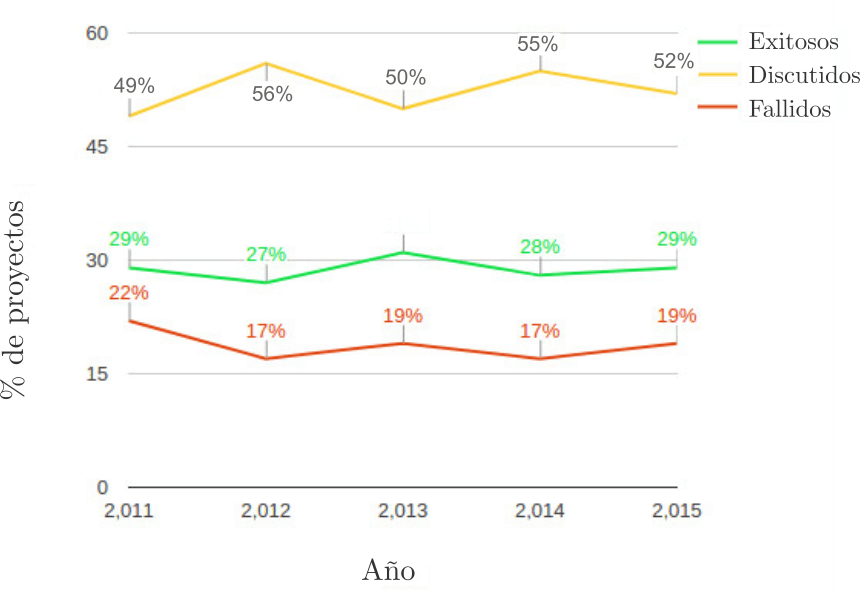
\includegraphics[width=11cm]{Img/Desarrollo/caos0.png}
\centering
\caption{\textbf{ \footnotesize{Proyectos, exitosos, discutidos y fallidos de 2011 hasta el 2015}}}
\label{fig:caos0}
\end{figure}

Lo primero que sorprende de esta comparativa es que del total de proyectos no hay ninguna tendencia en el éxito, se muestra oscilante sobre los mismos valores: el éxito entorno al 29\%, los discutidos entorno al 50\% y los fallidos entorno al 19\%. 

Hay otros factores para analizar que afectan al éxito o fracaso de los proyectos. Si se segmenta el informe por el tamaño de los proyectos como se puede apreciar en la Figura \ref{fig:caos1} , el resultado es claro e incluso esperado.
Se muestran los proyectos exitosos desde 2011 a 2015 desde la perspectiva del tamaño. El dato es muy significativo y confirma que más del 62\% de los proyectos exitosos son pequeños. Está claro que los proyectos grandes son exponencialmente más complejos que los proyectos pequeños y los proyectos gigantes son prácticamente imposibles de controlar.

\begin{figure}[h]
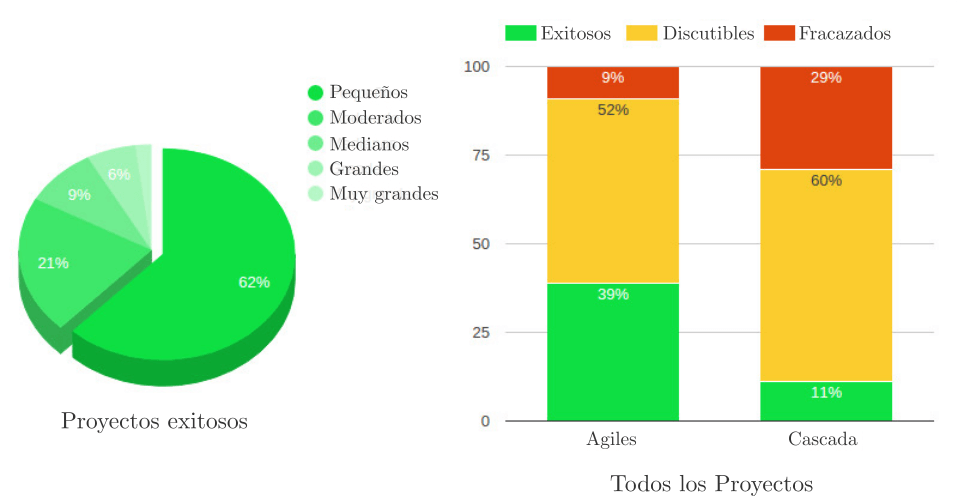
\includegraphics[width=15cm]{Img/Desarrollo/caos1.png}
\centering
\caption{\textbf{ \footnotesize{Éxito de los proyectos según su tamaño y métricas según la metodología.}}}
\label{fig:caos1}
\end{figure}

Otra información interesante que ofrece el Chaos Report es la comparativa del éxito de los proyectos en función de la metodología seguida para su desarrollo: \textit{ágil vs cascada}.

\begin{figure}[h]
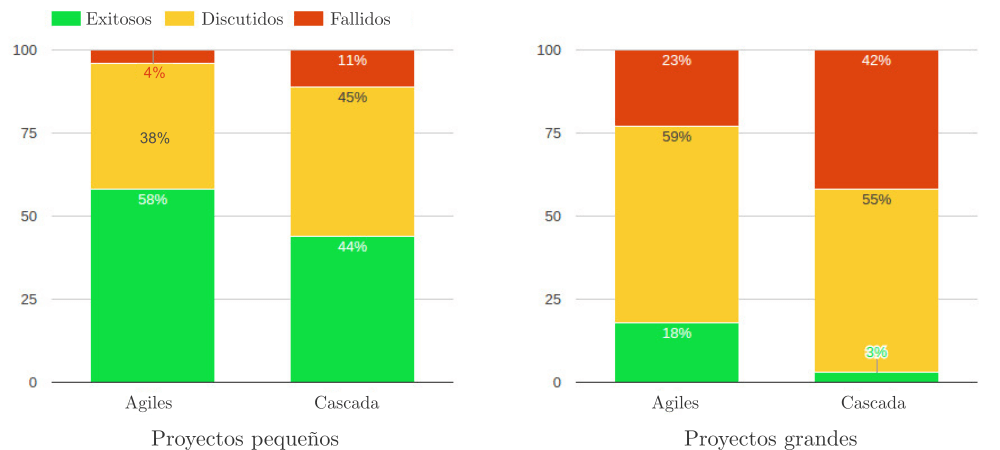
\includegraphics[width=15cm]{Img/Desarrollo/caos2.png}
\centering
\caption{\textbf{ \footnotesize{Métricas de los proyectos según la metodología.}}}
\label{fig:caos2}
\end{figure}

En los proyectos pequeños la diferencia no es tan grande pero es evidente. Los proyectos ágiles siguen siendo los más exitosos aunque por un margen menor. Ahora bien cuando el tamaño aumenta hacia proyectos grandes la diferencia se vuelve mucho más grande.

Al revisar los datos se debe considerar que hay muchos más proyectos en cascada que ágiles y que el dato que se muestra es relativo, es decir la muestra en ambos casos tiene distinto tamaño, por lo que puede ser un poco engañoso.
Aún así, por los datos presentados, los proyectos ágiles son mucho más éxitos que los no ágiles.\vskip
Con estos datos se puede ver que la metodología en sí no es el único motivo para la mejora del éxito de los proyectos sino que, si se divide el problema en partes más manejables, más pequeñas y se contruye progresivamente será más sencillo tener éxito.







https://www.infoq.com/articles/standish-chaos-2015

http://www.laboratorioti.com/2016/05/16/informe-del-caos-2015-chaos-report-2015-bien-mal-fueron-los-proyectos-ano-2015/

\subsection{Enfoque LEAN UX}
\label{section:pmv}
https://www.ida.cl/blog/estrategia-digital/principios-metodologia-lean-ux/
Los equipos de desarrollo de software en la actualidad utilizan técnicas como el desarrollo ágil, la integración continua y el despliegue continuo reduciendo drásticamente el tiempo para generar nuevas cambios en el software. Estos equipos realizan cambios en el código y suben los cambios a producción\footnote{Producción es la instancia del software cuando se encuentra a disposición de los usuarios finales.} con velocidad similar a la acción de guardar cualquier archivo en una computadora. Además, utilizan esos ciclos cortos como ventaja competitiva, producen nuevas versiones del software en tiempos acotados, lo que permite obtener retroalimentación del mercado e iterar incorporando lo que han aprendido y tal vez sin advertirlo aumentan las expectativas de los clientes que pueden obtener más calidad en menos tiempo. En este nuevo contexto, las prácticas de pensar todo al inicio de los procesos quedaron obsoletas. \vskip
\textit{Lean User Experience} (Lean UX) se puede traducir como \textit{Experiencia de Usuario\footnote{La experiencia de usuario es el conjunto de factores y elementos relativos a la interacción del usuario, con un entorno o dispositivo concretos, cuyo resultado es la generación de una percepción positiva o negativa de dicho servicio, producto o dispositivo.} limpia o sin desperdicios} y se describe como una nueva etapa evolutiva en el diseño de productos, de manera que se puedan solventar las prácticas de diseño obsoletas. Su objetivo es tomar las mejores herramientas del diseño y adaptarlas a esta nueva realidad. \citep{Gothelf2013}

Lean UX es profundamente colaborativo, en gran medida porque:
\begin{itemize}

    \item Logra que los diseñadores no están aislados del resto del equipo de trabajo.
    \item Permite implementar técnicas para construir una comprensión compartida del proyecto. 
    \item Logra un clima propicio para la retroalimentación con los usuarios finales y  replantea las conversaciones de diseño en términos objetivos, se pueden obtener métricas sobre las funcionalidades, analizar y ajustar.
    \item Cambia la forma en que se comunica el diseño del producto: en lugar de comunicar características y documentos exhaustivos se puede comunicar funcionalidad.
\end{itemize}

 
\vskip


Los 3 pilares principales de Lean UX son:
\begin{enumerate}
    \item \textbf{Design Thinking o Pensamiento de Diseño} \vskip
    Alienta al equipo a colaborar en todas las etapas del proyecto y a considerar el producto desde una perspectiva global, utilizando la sensibilidad y los métodos de los diseñadores para satisfacer las necesidades del usuario final con soluciones tecnológicamente viables.

    \item \textbf{Desarrollo Ágil}\vskip
     Aplica los cuatro principios básicos del desarrollo Ágil al diseño de los productos.
        
\begin{itemize}
\item
\textbf{Los individuos y las interacciones son más importantes que los procesos y las herramientas}\vskip
Para generar rápidamente las mejores soluciones, es necesario implicar al todo el equipo. El intercambio de ideas deberá ser libre y frecuente. La conversación fluida entre colegas deberá primar por encima de las restricciones propias de las herramientas, ya sea en los procesos o en la producción.
\item
\textbf{El software funcional es más importante que la documentación exhaustiva}\vskip
Se pueden encontrar múltiples soluciones para todos los problemas de negocio y todos los miembros del equipo podrán tener una opinión diferente de cuál es la mejor. El reto está en averiguar cuál de ellas es la que tiene más posibilidades. Por eso, cuanto antes se cuente con un software que funcione, antes se puede encontrar la solución que mejor se adapte a los requerimientos.
\item
\textbf{La colaboración con los clientes es más importante que la negociación de contratos con ellos}\vskip
Si el equipo colabora con los usuarios/clientes, hay un entendimiento común sobre los problemas y las posibles soluciones. Cualquier decisión que se adopte después se tomará por consenso, lo que se traduce en iteraciones más rápidas y una verdadera implicación de todos los actores con la ventaja de trabajar siempre con soluciones validadas. Además, como todos los miembros del equipo participan en la toma de decisiones, no se requieren tantas entregas de documentación por escrito.
\item
\textbf{La respuesta a los cambios es más importante que la planificación}\vskip
Lean UX asume que los diseñadores del producto inicial no encontrarán la solución a la primera, por lo que el objetivo consiste en averiguar qué han hecho mal lo antes posible. Una vez que se descubra lo que funciona y lo que no, se pueden ajustar las propuestas y volver a probarlas. Así, la retroalimentación mantendrá ágil al equipo, dirigiendo la solución siempre en la dirección correcta.
\end{itemize}

\item \textbf{Método Lean Startup}\vskip Utiliza un bucle de retroalimentación llamado  ``Construir-Medir-Aprender" para minimizar el riesgo del proyecto, haciendo que los equipos construyan y aprendan rápidamente.
Los equipos construyen productos viables mínimos en inglés \textit{Minimum Viable Product} (MVP) y los envían para comenzar el proceso de aprendizaje tan pronto como sea posible. En la Figura \ref{fig:leanux} se puede apreciar el proceso.\vskip
Lean Startup\footnote{\url{https://es.wikipedia.org/wiki/Lean_startup} } es una filosofía inspirada en \textit{Lean Manufacturing}\footnote{\url{https://es.wikipedia.org/wiki/Lean_manufacturing}} que desde el principio aboga por la creación de prototipos rápidos para comprobar, por un lado, que las suposiciones son correctas y, por otro, para conseguir retroalimentación de los usuarios de forma inmediata y así poder mejorar el software más rápido que las prácticas tradicionales de ingeniería de software.\vskip
Lean UX, por su parte, es una implementación directa de esta filosofía aplicada al diseño de productos. Cada diseño es una solución propuesta, una hipótesis. Su objetivo consiste en validar la solución de la manera más eficiente posible mediante la realimentación. El componente más pequeño que se puede construir para probar cada hipótesis es el Producto Viable Mínimo MVP. 
\end{enumerate}


\begin{figure}[h]
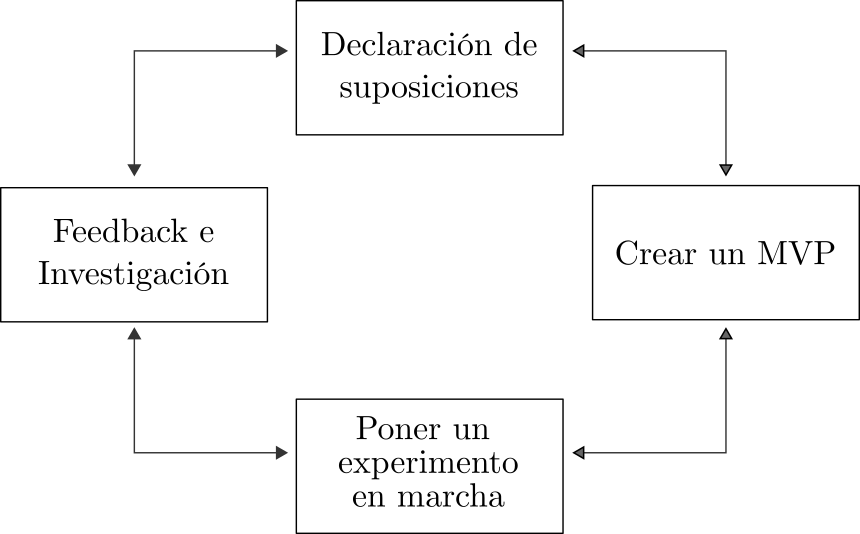
\includegraphics[width=10cm]{Img/Desarrollo/desarrollo0.png}
\centering
\caption{\textbf{ \footnotesize{Proceso del enfoque LEAN UX. }}}
\end{figure}
\label{fig:leanux}

Lean UX funciona como una práctica para entender rápidamente la función de un producto. Para ello elije un camino colaborativo y multidisciplinario; reduce el énfasis por la documentación exhaustiva y aumenta el enfoque en la construcción de un entendimiento compartido del producto que está siendo diseñado. Como consecuencia de usar este enfoque se obtiene: un equipo que trabaja de forma colaborativa, iterativamente, reduciendo al mínimo los documentos entregables, enfocándose en el software funcional y en la retroalimentación con el usuario final.

\subsubsection{Principios de LEAN UX}
\textit{Lean UX} contiene en su núcleo un juego de principios clave, que abarcan el proceso de diseño, la colaboración, la gestión, etc., para que los equipos puedan sacarle el máximo provecho al enfoque propio de la metodología. Se consigue con ellos que los equipos se encaminen en la dirección correcta y sean especialmente útiles para implementar los procesos de Lean UX. Los procesos, sin duda se deben ajustar a cada proyecto, por ende los principios de utilizan como guía y no de forma obligatoria. Algunos de ellos serán más difíciles de implementar y su impacto será mayor. Los equipos adoptarán sin problema otros, pero, independientemente de las dificultades, todos ellos ayudan a crear una organización más colaborativa, multifuncional y adaptada a la realidad actual de los proyectos.\vskip

A continuación se detallan los principios:
\begin{itemize}
    \item \textbf{Principio: Equipos multifuncionales}\vskip 
    ¿De qué se trata? Los equipos multifuncionales deben incluir todas las disciplinas que intervienen en la creación del producto. La ingeniería del software, la gestión del producto, el diseño de interacciones, el diseño gráfico, la estrategia de contenidos y el control de calidad (QA), todas deben contar con representantes en ellos. Lean UX necesita que todos los que se dedican a estos campos colaboren intensamente, por lo que la implicación del equipo debe ser continua, desde el primer día del proyecto hasta el final.\vskip
    ¿Por qué hacerlo? Estos equipos, diversos en su constitución, evitan el desarrollo en cascada, con su proceso rígido de entregas de documentación. En su lugar, todos los campos aportan conocimiento mucho antes al proceso. Como la metodología promueve, además, que los miembros de los diferentes ámbitos hablen entre ellos, la eficacia del equipo aumenta.
    
\item \textbf{Principio: Pequeños, dedicados, coubicados }\vskip 
    ¿De qué se trata? Es necesario limitar el tamaño de los equipos, no deben ser mayores de diez personas, dedicados exclusivamente al proyecto y trabajando en el mismo lugar. \vskip
    ¿Por qué hacerlo? El beneficio de los equipos pequeños se resume en tres palabras: comunicación, concentración y camaradería. Así se comunica de forma sencilla sobre el estado del proyecto, de los cambios y del nuevo conocimiento que surja. La dedicación en exclusiva, por otra parte, hace que todos los miembros estén centrados en las mismas prioridades. Y además, trabajar en el mismo lugar hace las relaciones entre colegas sean más estrechas.
    
    \item \textbf{Principio: Equipos centrados en los problemas}\vskip
    ¿De qué se trata? Un equipo centrado en los problemas es un grupo que sabe que debe resolver el problema asignado y no limitarse a implementar un grupo de funciones. Este principio es una extensión lógica del anterior, que afirmaba que el progreso del proyecto dependía de los resultados.\vskip
    ¿Por qué hacerlo? Si se asignan problemas completos a un equipo se demuestra más confianza en las personas que lo conforman. Además, así se les permite llegar a sus propias soluciones, con lo que se consigue aumentar la sensación de pertenencia en el proyecto.
    
    \item \textbf{Principio: Eliminación del despilfarro}\vskip
    ¿De qué se trata? Una de los prácticas principales de \textit{Lean manufacturing} es la eliminación de todo lo que no contribuya a conseguir el objetivo final. En Lean UX, este objetivo final es la producción de mejores resultados, por lo que todo lo que no ayude a conseguirlos se considera despilfarro y debe eliminarse del proceso de trabajo del equipo.\vskip
    ¿Por qué hacerlo? Los recursos del equipo son limitados, por lo que cuanto más despilfarro se elimine, más rápido podrán producir sus miembros. En realidad, lo que los equipos necesitan es ser efectivos y trabajar en los retos adecuados. Si se elimina el despilfarro, la atención de los equipos estará centrada donde se debe.
    
    \item \textbf{Principio: Lotes pequeños}\vskip
    ¿De qué se trata? Otra idea fundamental de \textit{Lean manufacturing} es la utilización de lotes pequeños. En ese modelo, esta noción se usa para indicar que no se deben tener muchos productos en stock y que la calidad de producción debía ser alta. Adaptado a Lean UX, su significado es que el equipo solo debe crear los diseños necesarios para avanzar, evitando crear un gran stock de ideas de diseño sin probar ni implementar. \vskip
    ¿Por qué hacerlo? El diseño en grandes lotes resta eficiencia al equipo, ya que, para poder realizar grandes entregas de diseño, se insume mucho tiempo. En ese tiempo no se puede aprender si las ideas funcionan e, inevitablemente, algunos de los miembros tendrán que estar desocupados, aparte de generar recursos de diseño inútiles. Es decir, se trata de una estrategia con un despilfarro que no maximiza el potencial de aprendizaje del equipo.
    
    \item \textbf{Principio: Descubrimiento continuo }\vskip
    ¿De qué se trata? El descubrimiento continuo consiste en comprometer a los usuarios con el proceso de diseño y desarrollo, mediante actividades programadas con ellos en intervalos regulares, en las que se aplican métodos cualitativos y cuantitativos. El objetivo es entender lo que los usuarios hacen con productos y por qué lo hacen. La investigación con ellos debe realizarse de forma frecuente y regular y debe implicar al todo el equipo.\vskip
    ¿Por qué hacerlo? Las conversaciones regulares con los usuarios ofrecen oportunidades de validar nuevas ideas sobre el producto. Por otra parte, al incluir al equipo completo en el ciclo de desarrollo, estos desarrollarán empatía por los usuarios y por los problemas a los que tienen que enfrentarse. Además, como todos los miembros aprenden juntos en las reuniones, no será necesario generar demasiada documentación ni explicar lo sucedido en otras reuniones internas.
    
    \item \textbf{Principio: GOOB: La nueva centralidad del usuario}\vskip
    ¿De qué se trata? Se utiliza el acrónimo \textit{Salir del edificio} en ingles \textit{Getting Out Of the Building} (GOOB). Quiere decir que los debates sobre las necesidades de los usuarios no tienen por qué cerrarse en el mismo lugar en el que se desarrollan, es decir, en la oficina. Las respuestas, más bien, están en el mercado, fuera de ella. Después de mucho tiempo abogando por la investigación del comportamiento de los usuarios, la comunidad de experiencia de usuarios (UX) tiene un aliado en Steve Blank, que viene del mundo de los negocios. Su consejo: Ofrecer la posibilidad a los usuarios de dar su opinión sobre las ideas mucho antes de lo que lo han hecho en el pasado. Mucho antes. Brindar nociones de la realidad mientras aún se está en etapas prematuras de desarrollo. Es mucho mejor averiguar que las ideas no son correctas mucho antes de dedicar tiempo y recursos a construir un producto que nadie quiere o necesota.\vskip
    ¿Por qué hacerlo? En los últimos tiempos, el éxito o el fracaso de los productos no dependen de las decisiones del equipo de desarrollo, sino de los usuarios. Son ellos los que tendrán que utilizar los producto. Cuanto antes se los haga participar, antes se aprende si las ideas están listas para pasar a la fase de desarrollo.

    \item \textbf{Principio: Entendimiento común}\vskip 
    ¿De qué se trata? El entendimiento común es el conocimiento colectivo del equipo. Se construye poco a poco a medida que ese equipo trabaja de forma conjunta y consiste en una comprensión profunda del espacio, del producto y de los clientes.\vskip 
    ¿Por qué hacerlo? Este tipo de conocimiento es la moneda de cambio de Lean UX. Cuanto más sepa el equipo, como colectivo, de lo que está haciendo y de por qué lo está haciendo, menos dependerá de informes de segunda mano y de documentos detallados para continuar con su trabajo.
    
    \item \textbf{Principio: Antimodelos: estrellas, gurús y ninjas }\vskip 
    ¿De qué se trata? Lean UX aboga por una mentalidad de equipo. Las estrellas, los gurús, los ninjas y, en general, rompen la cohesión del equipo y reducen la colaboración.\vskip ¿Por qué hacerlo? Las estrellas no comparten las ideas ni la atención de los demás. Si se cuenta con individuos de este tipo en los equipos, con grandes egos y determinados a brillar por encima de todos, se rompe la colaboración del grupo. Si eso sucede no se cuenta con un entorno en el que se pueda construir un entendimiento común, necesario para avanzar de forma efectiva.
    
    \item \textbf{Principio:Exteriorización del trabajo}\vskip
    ¿De qué se trata? Con exteriorización me refiero a exponer el trabajo de forma pública, más allá de las computadoras. Los equipos pueden utilizar pizarras, tableros de cartón, paredes repletas de artefactos, salidas impresas, notas adhesivas, lo que sea que hayan utilizado para reflejar sus ideas, para poder mostrar el trabajo a compañeros, colegas y clientes.\vskip 
    ¿Por qué hacerlo? La exteriorización somete las ideas a escrutinio público y así todos los miembros del equipo pueden ver dónde se encuentran como grupo. De esta manera se crea un flujo de información que circula entre todos los miembros, información que está en el ambiente y que inspira nuevas ideas, construidas sobre las que se han compartido. Además, esta forma de trabajar hace participar a todos los miembros del equipo, incluso las personas tímidas, ya que las notas adhesivas, se tratan por igual.

    \item \textbf{Principio: Aprendizaje en lugar de crecimiento}\vskip
    ¿De qué se trata? Es complicado concebir una buena idea y hacerla crecer al mismo tiempo. Son actividades contradictorias. Lean UX apuesta por que, en primer lugar, se concentre en el aprendizaje y luego en su crecimiento.\vskip 
    ¿Por qué hacerlo? Escalar una idea que no se ha probado es arriesgado. Podría funcionar o podría no hacerlo. Si no lo hace y la idea se sube a producción para todos los usuario, en lugar de para unos cuantos con los que probar, el equipo habrá perdido tiempo y recursos valiosos en hacerlo. Al asegurarse de que una idea funciona antes de hacerla crecer, se reduce el riesgo que conllevan los grandes despliegues de funciones.
    
    \item \textbf{Principio: Permiso para equivocarse}\vskip
    ¿De qué se trata? Para encontrar las mejores soluciones a los problemas, los equipos Lean UX necesitan experimentar con las ideas. La mayoría de estas ideas no funcionarán en primera instancia, por lo que, si se necesita que sean exitosas, el equipo debe sentirse libre para equivocarse. Este permiso significa que puede contar con un entorno seguro en el que experimentar, una filosofía que se debe aplicar tanto al entorno técnico (deben ser capaces de generar ideas en un entorno seguro) como al cultural (nadie debe penalizar a un miembro del equipo por probar ideas que no funcionen).\vskip 
    ¿Por qué hacerlo? El permiso para equivocarse alimenta la cultura de la experimentación que, a su vez, da alas a la creatividad. La creatividad, por su parte, hace que aparezcan soluciones innovadoras. Cuando, al equivocarse, los equipos no tienen miedo de ser penalizados, estarán dispuestos a correr riesgos. Y las grandes ideas siempre proceden de los riesgos.
    
    \item \textbf{Principio: Escapar de los negocios basados en entregables }\vskip
    ¿De qué se trata? El progreso de un proyecto depende de los resultados que se consiguen, no de los documentos que el equipo escriba. Por otra parte, la colaboración multifuncional permite conseguir que los participantes del proyecto tengan más en cuenta los resultados y menos los artefactos que se estén creando.\vskip 
    ¿Por qué hacerlo? Los documentos no solucionan los problemas de los usuarios; lo hacen los buenos productos. La atención del equipo debe estar enfocada en qué funciones de las que está desarrollando tienen mayor impacto. Los procedimientos que el equipo utilice para llegar a ese conocimiento son irrelevantes. Lo que importa es la calidad del producto, medida como la reacción que el usuario presenta ante él.
    
\end{itemize}



Los principios fundacionales de Lean UX tratan de los atributos principales que debe tener cualquier equipo que trabaje con esta metodología.
Por todo lo señalado se considera que este enfoque es el adecuado para abordar el trabajo en la aplicación COCADA para los métodos de trabajo en equipo.
Las etapas de LEAN UX se pueden ver aplicadas en este documento en el siguiente capítulo correspondiente al desarrollo del prototipo.



Agregar lo de chaos report http://www.laboratorioti.com/2016/05/16/informe-del-caos-2015-chaos-report-2015-bien-mal-fueron-los-proyectos-ano-2015/

https://modelometodoygestion.wordpress.com/2017/02/21/chaos-report-15-scrum/

Ver frase final para chamu
http://www.uxline.com/blog/agile-ux-versus-lean-ux/



VER LO DE FUZZY DESIGN y agregar tambien a la parte de codiseño

https://blog.prototypr.io/the-teapot-model-how-to-explain-a-fuzzy-design-process-to-anxious-clients-4a2e8487bc87


COMO ENGANCHAR TODO
https://es.linkedin.com/pulse/design-thinking-lean-startup-agile-victor-mansilla


https://www.cio.com/article/3174516/project-management/it-project-success-rates-finally-improving.html



https://www.pmi.org/-/media/pmi/documents/public/pdf/learning/thought-leadership/pulse/pulse-of-the-profession-2017.pdf


\section{Antecedentes Tecnológicos}

\subsection{Modelado sólido en programas de diseño 3D}
Existen muchos programas con herramientas para el modelado sólido y booleano como el caso de Blender\footnote{\url{http://blender.org}}, un programa informático FLOOS multiplataforma, dedicado especialmente al modelado, iluminación, renderizado, animación y creación de gráficos 3D. También puede realizar composición digital, edición de vídeo, escultura y pintura digital. Entre todas sus características provee mecanismos para asegurar que los modelos sean sólidos.

\subsubsection{Geometría non-manifold en Blender}

\textit{Se considera non-manifold una geometría que no puede ser representada en el mundo real}, para ver en detalle los conceptos se puede ver la sección 2.4.2

\begin{figure}[h]
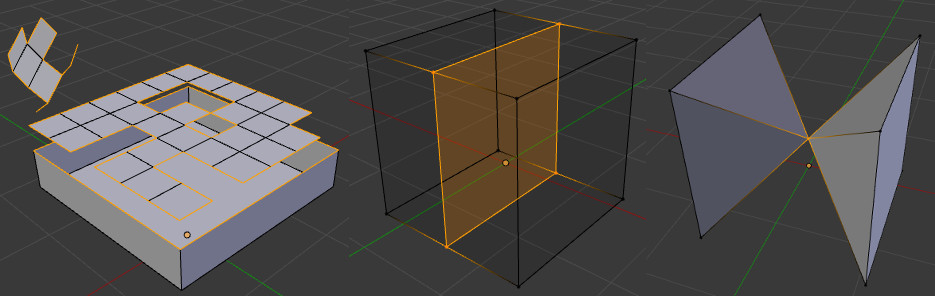
\includegraphics[width=12cm]{Img/Modelos/modelado20.jpg}
\centering
\caption{\textbf{ \footnotesize{Objetos no sólidos por geometria non-manifold en Blender. Caras y vértices sin conectar, Caras en el interior, Superficies sin grosor.}}}
\end{figure}


Para explicar una solución utilizaremos la Figura \ref{fig:blender} que se muestra a continuación. El modelo 3D de la izquierda no consiste en un volumen, sino en una serie de superficies que no están cerradas y no posee grosor. Para garantizar que el objeto sea sólido es importante cerrar los agujeros en el modelo. Esto es posible creando una superficie con $N$ caras como vemos en el resultado de la derecha.

\begin{figure}[h]
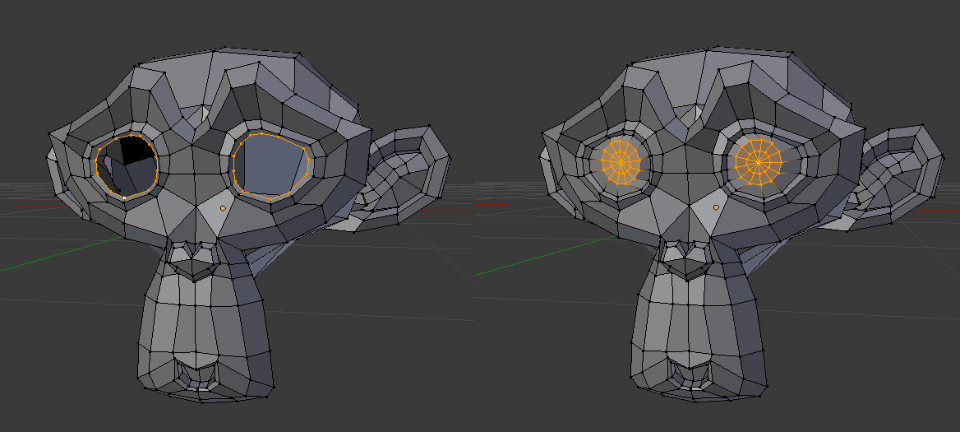
\includegraphics[width=10cm]{Img/Modelos/modelado21.jpg}
\centering
\caption{\textbf{ \footnotesize{Objetos no sólido por superficies no cerradas y su solución }}}
\label{fig:blender}
\end{figure}

\vspace{5mm}
\subsubsection{Modelado booleano en Blender}

Lo recomendado en Blender es usar un Modificador\footnote{
Los modificadores en Blender son operaciones automáticas que afectan a un objeto de una manera no destructiva.} Booleano para tener mayor flexibilidad y realizar ediciones no destructivas. Mediante los modificadores se pueden mover los objetos y ver el operador booleano (union, intersección o diferencia) aplicado de forma interactiva en tiempo real.

\begin{figure}[h]
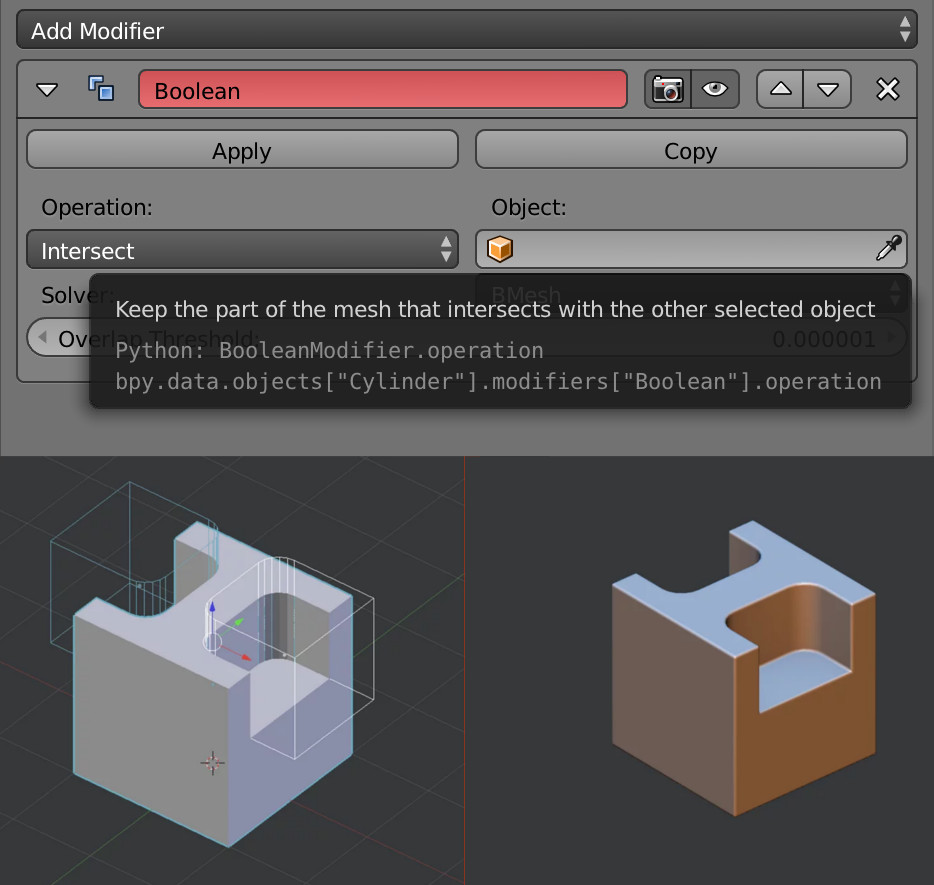
\includegraphics[width=9cm]{Img/Modelos/modelado22.jpg}
\centering
\caption{\textbf{ \footnotesize{Modificador booleano, aplicación de intersecciones y su resultado. }}}
\end{figure}

La herramienta booleana nativa de Blender es excelente para partes simples o de modelado mecánico con resultados en tiempo real. Con complementos en inglés \textit{add-ons} se puede extender la aplicación booleana a modelos con mallas complejas, con muchos polígonos y que requieren una elevada potencia de cálculo.
Cork\footnote{\url{https://github.com/dfelinto/cork-on-blender}} es un complemento para Blender que se desarrolló especialmente para el ámbito de la impresión 3D. En la Figura \ref{fig:cork} se puede ver un ejemplo de su potencia en operaciones booleanas aplicado a casos reales de medicina.

\begin{figure}[h]
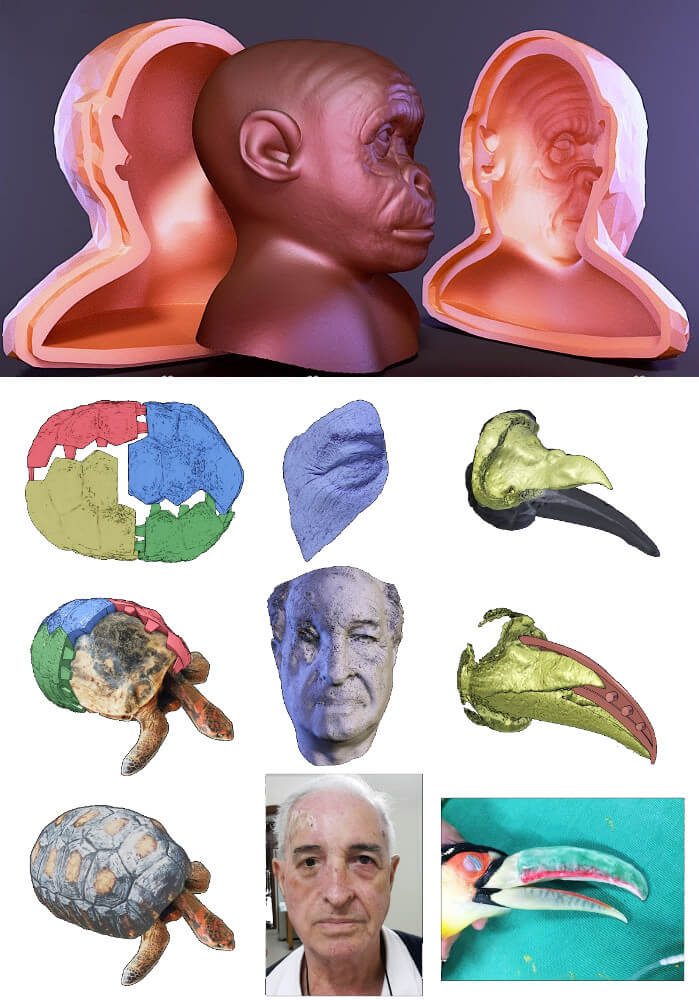
\includegraphics[width=12cm]{Img/Modelos/corkc.jpg}
\centering
\caption{\textbf{ \footnotesize{Ejemplo de modificadores booleanos con el add-on Cork y aplicaciones reales de prótesis médicas.   }}}
\label{fig:cork}
\end{figure}





\clearpage

\subsection{Programas para diseño especificado en algoritmos}
Las interfaces de scripting explicadas en la secciónXX, utilizadas para definir diseños paramétricos se puede encontrar en programas como OpenSCAD\footnote{\url{http://www.openscad.org/}}, una aplicación FLOSS para crear objetos sólidos de CAD utilizando geometría constructiva de sólidos (CSG). No es un editor interactivo sino un compilador 3D basado en un lenguaje de descripción textual. Un documento de OpenSCAD especifica primitivas geométricas y define como son modificadas y manipuladas para reproducir un modelo 3D.

En la última década se ha visto la aparición de un nuevo tipo de interfaz de secuencias de comandos, la interfaz visual. La programación visual implica representar programas no como texto, sino como diagramas. Un ejemplo es Grasshopper \footnote{ \url{http://www.grasshopper3d.com/}} que se basa en gráficos que mapean el flujo de relaciones desde parámetros, a través de funciones definidas por el usuario, concluyendo normalmente con la generación de geometría. Los cambios en los parámetros o las relaciones del modelo hacen que los cambios se propaguen a través de las funciones explícitas para volver a dibujar automáticamente la geometría. Como tal, son otra forma de crear un modelo paramétrico.


\begin{figure}[h]
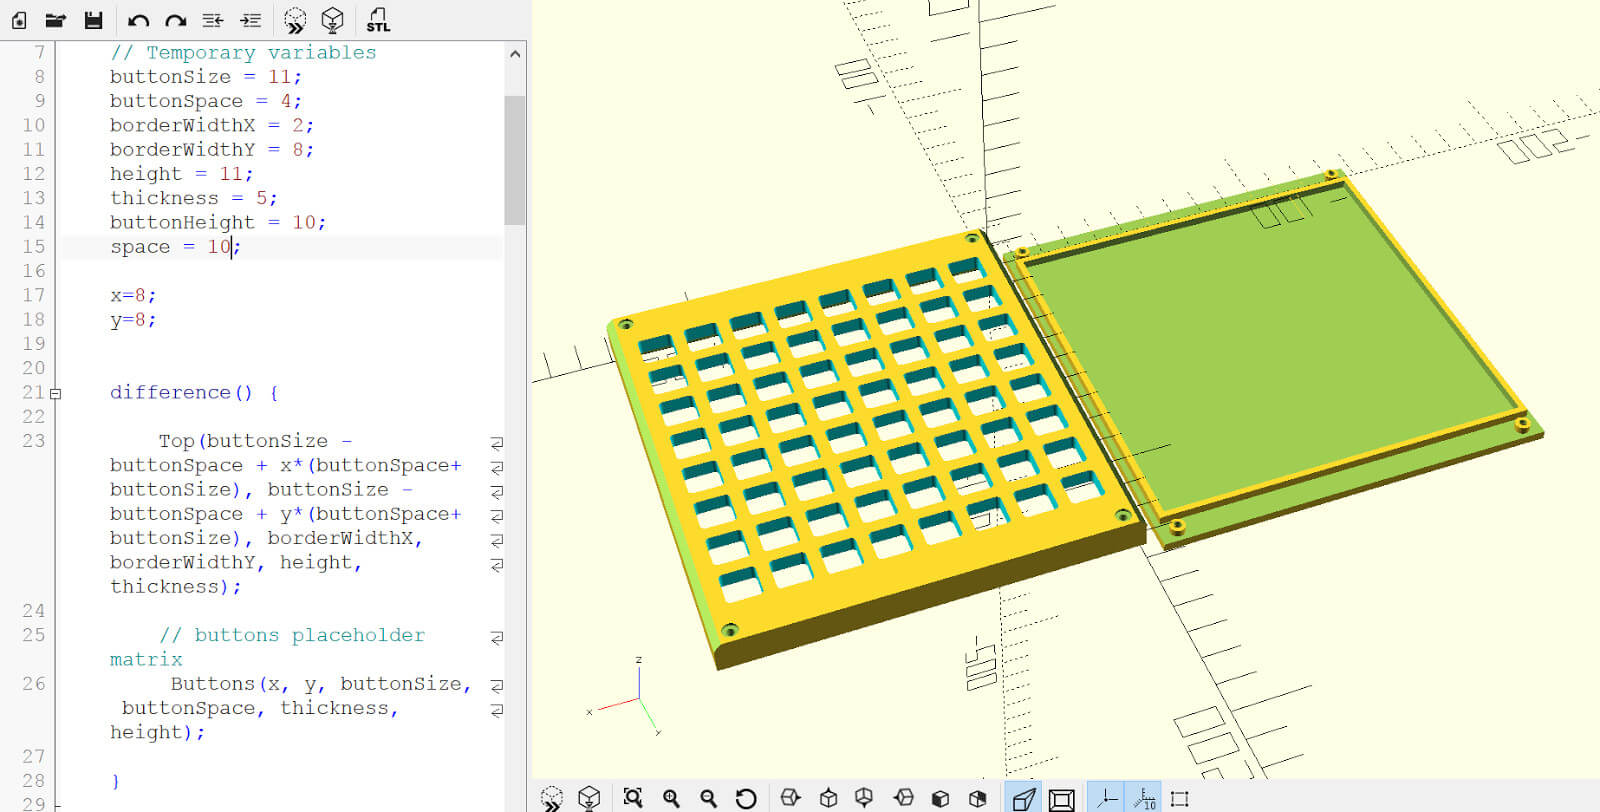
\includegraphics[width=14cm]{Img/CPD/openscadc.jpg}
\centering
\caption{\textbf{\footnotesize{Interfaz de OpenSCAD con el código que genera el modelo 3D}}}
\end{figure}

\begin{figure}[h]
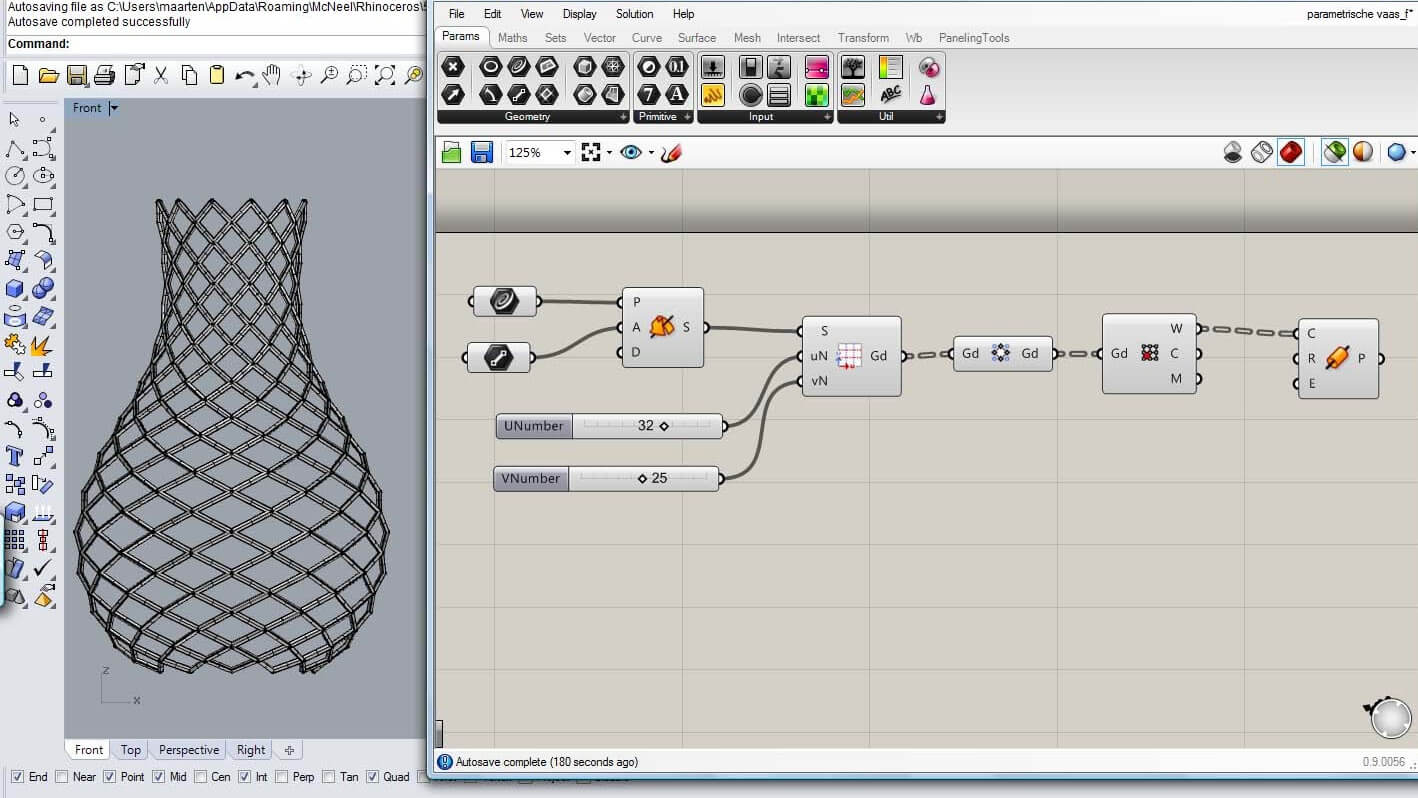
\includegraphics[width=14cm]{Img/CPD/rhinoc.jpg}
\centering
\caption{\textbf{\footnotesize{Rhinoceros con Graphopper, a la derecha se puede ver el diagrama que genera el modelo 3D}}}
\end{figure}

\subsection{Modelado booleano especificado en algoritmos, DEJAR PARA DESARROLLO}

El lenguaje de descripción debe proveer los mecanismos para crear y manipular sólidos en 3D, así también formas en 2D para poder producir modelos de barrido (extrusión) o bien nuevas primitivas a través de la intersección. El  modelado  booleano  es  un proceso  descriptivo,  es  decir,  sólo  se limita  a  especificar que primitivas se utilizan y cómo se combinan, para una mejor comprensión se utiliza un pseudocódigo\footnote{Un pseudocódigo (o falso lenguaje) es una descripción de alto nivel compacta e informal del principio operativo de un algoritmo} similar al lenguaje descriptivo de OpenSCAD.

\textbf{Objetos}. Los Objetos representan la construcción de los modelos, creados a partir  de las primitivas. Los objetos pueden utilizar uno o más parámetros por lo tanto se pueden especificar utilizando paréntesis \textbf{( )}

\begin{minted}[baselinestretch=1]{python}
   objeto()
\end{minted}


\textbf{Operadores}. Los Operadores o Transformaciones sirven para modificar la escala, rotación y aplicar otras operaciones sobre los objetos. Los Operadores pueden recibir uno o más parámetros utilizando paréntesis \textbf{()}

\begin{minted}[baselinestretch=1]{python}
   operador()
\end{minted}


\textbf{Parámetros}. Los parámetros o acciones sirven para construir objetos y definir operadores. Pueden ser asignados de forma directa utilizando variables.

\begin{minted}[baselinestretch=1]{python}
   parametro
   var a = parametro
\end{minted}

\textbf{Comentarios}. Sirve para agregar texto informativo sin que el mismo afecte al funcionamiento del código del programa. Se especifica con numeral \# seguido del texto.
\begin{minted}[baselinestretch=1, 
framesep=0]{python}
    # esto es un comentario
\end{minted}

\vspace{5mm}
Un ejemplo de utilización del pseudocódigo, ver resultado en la Figura \ref{fig:traslacion}

\begin{minted}[baselinestretch=1, framesep=0]{python}
    # objeto(parametro1, ...).operador(parametro2, parametro3, ...)
    b = cubo(10, 10, 20).trasladar(15, 0, 2) 
\end{minted}


\clearpage
\subsubsection{Cubo especificado en algoritmos}
\begin{description}
\item  \textbf{Parámetros:}
\item   \textbf{longitud}:
\begin{description}
\item \textbf{1 valor} único que especifica la longitud de todos los lados del cubo.
\item \textbf{3 valores} en un vector $[x,y,z]$, especificando dimensiones $x$, $y$ y $z$.
\end{description}
\item   \textbf{centro}:
\begin{description}
\item \textbf{F} falso (por defecto), 1er octante positivo, esquina en $(0, 0, 0)$
\item \textbf{V} Verdadero, el centro del cubo está en $(0, 0, 0)$
\end{description}
\end{description}

Ver aplicación en los ejemplos a y b:

\textbf{a)} Todos los scripts (lineas de código) son equivalentes en este ejemplo: \begin{listing}[ht]
\begin{minted}[baselinestretch=1]{python}
        cubo(longitud=8)
        cubo(8)
        cubo([8, 8, 8])
         
        cubo(8, F)
        cubo([8, 8, 8], F)
        cubo([8, 8, 8], centro=F)
        cubo(longitud=[8, 8, 8], centro=F)
        cubo(centro=F, longitud=[8, 8, 8])
\end{minted}
\end{listing}

\begin{figure}[h]
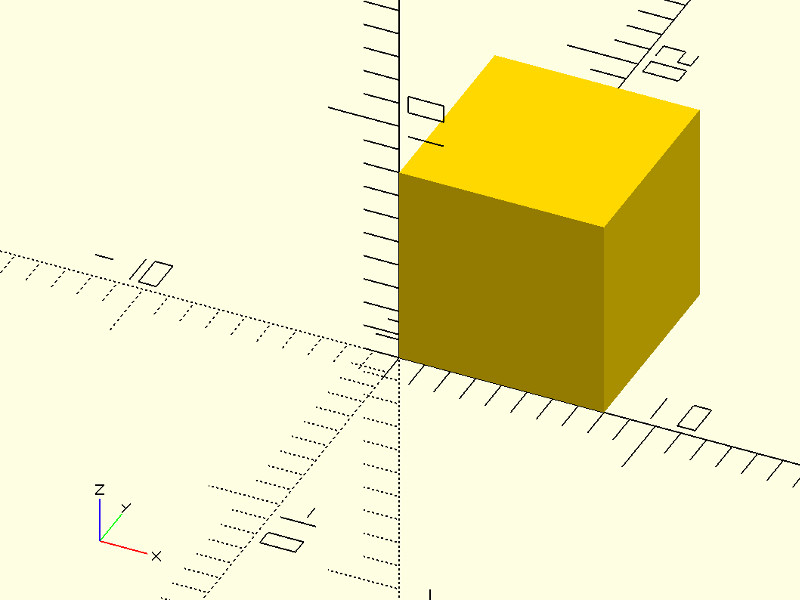
\includegraphics[width=7cm]{Img/Modelos/modelado1.jpg}
\centering
\caption{\textbf{\footnotesize{Cubo de $longitud = 8$ y ubicado en la esquina $(0,\ 0, \ 0)$. }}}
\end{figure}


\clearpage
\textbf{b)} Todos los scripts (lineas de código) son equivalentes en este ejemplo: \begin{listing}[ht]
\begin{minted}[baselinestretch=1]{python}
    cubo([18, 28, 8], centro=V)
    caja=[18, 28, 8] cubo(caja, V)
\end{minted}
\end{listing}

\begin{figure}[h]
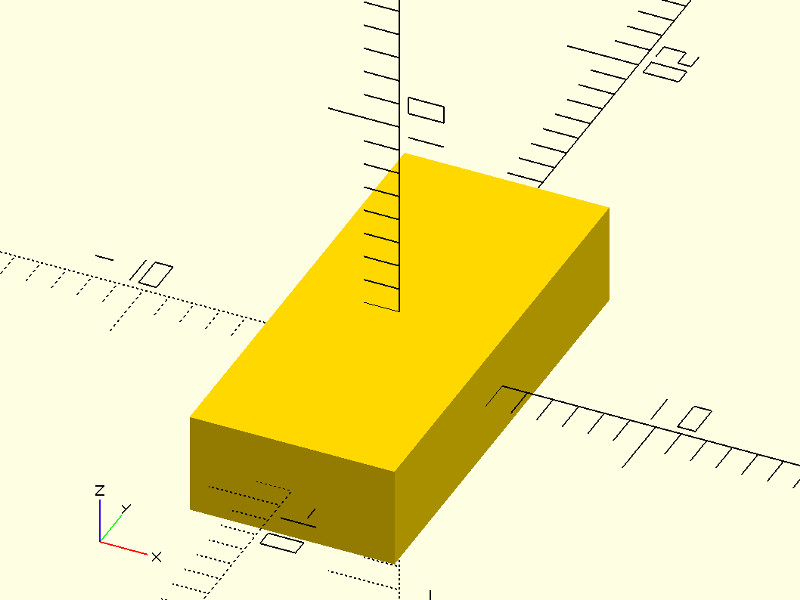
\includegraphics[width=7cm]{Img/Modelos/modelado2.jpg}
\centering
\caption{\textbf{\footnotesize{prisma rectangular construido a partir de un cubo. }}}
\end{figure}

\clearpage
\subsubsection{Esfera especificada en algoritmos}

\begin{description}
\item \textbf{Parámetros:}
\item  \textbf{r}: Radio de la esfera.
\item  \textbf{d}: Diámetro de la esfera.
\item  \textbf{res}: Resolución de la esfera.
\end{description}

\textbf{a)} 

\begin{minted}{python}
    esfera(r=6, res=12); 
\end{minted}


\begin{figure}[h]
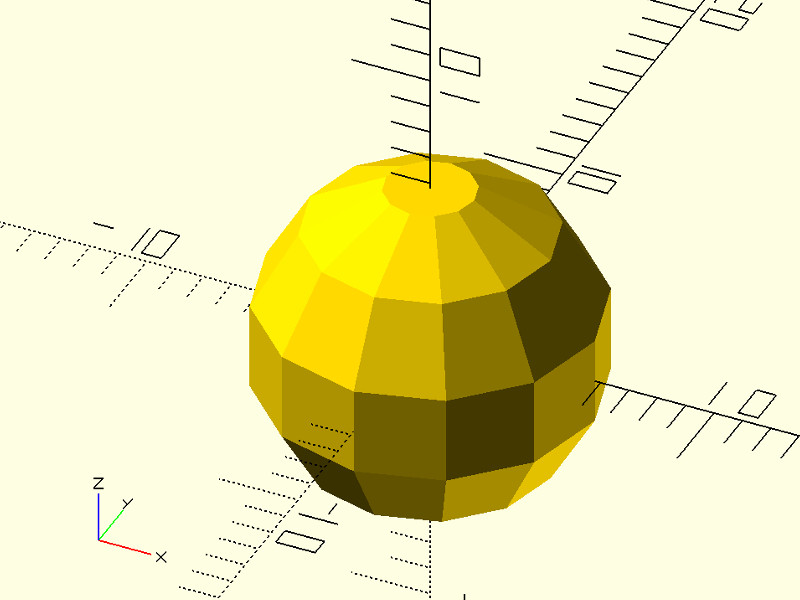
\includegraphics[width=7cm]{Img/Modelos/modelado3.jpg}
\centering
\caption{\textbf{\footnotesize{Esfera de $radio=6$ con baja resolución (12 polígonos en $360^\circ)$. }}}
\end{figure}

\textbf{b)} 

\begin{minted}{python}
    esfera(r=8, res=100); 
\end{minted}

\begin{figure}[h]
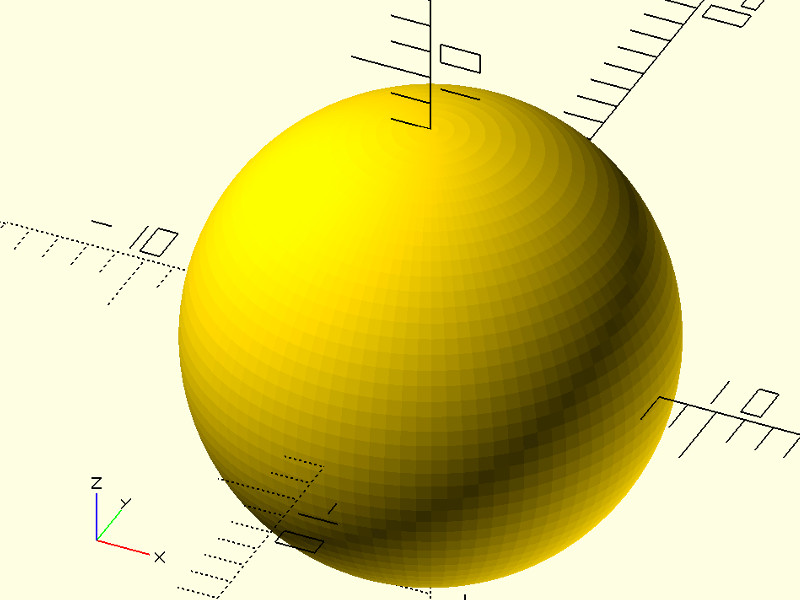
\includegraphics[width=7cm]{Img/Modelos/modelado4.jpg}
\centering
\caption{\textbf{ \footnotesize{Esfera de $radio=8$ con alta resolución (100 polígonos en $360^\circ$).}}}
\end{figure}

\clearpage
\subsubsection{Cilindro especificado en algoritmos}
\begin{description}
\item  \textbf{Parámetros:}
\item  \textbf{alto}: Alto del cilindro o cono.
\item  \textbf{r}: Radio del cilindro cuando r1 = r2.
\item  \textbf{r1}: Radio inferior.
\item  \textbf{r2}: Radio superior.
\item  \textbf{d1}: Diámetro inferior.
\item  \textbf{d2}: Diámetro superior.
\item   \textbf{centro}:
\begin{description}
\item \textbf{F} falso (por defecto), Inicia en el $z$ desde $0$ hasta $alto$
\item \textbf{V} Verdadero, sobre el eje Z en el rango $-alto/2$ hasta $alto/2$

\end{description}
\item \textbf{res}: Resolución de la esfera.
\end{description}

Ver aplicación en los ejemplos a y b:

\textbf{a)} Todos los scripts son equivalentes para este ejemplo:


\begin{minted}[baselinestretch=1]{python}
    cilindro(alto=15, r1=9.5, r2=19.5, centro=F)
    cilindro(15, 9.5, 19.5, F)
    cilindro(15, 9.5, 19.5)
    cilindro(15, 9.5, d2=39)
    cilindro(15, d1=19, d2=39)
    cilindro(15, d1=19, r2=19.5)
\end{minted}


\begin{figure}[h]
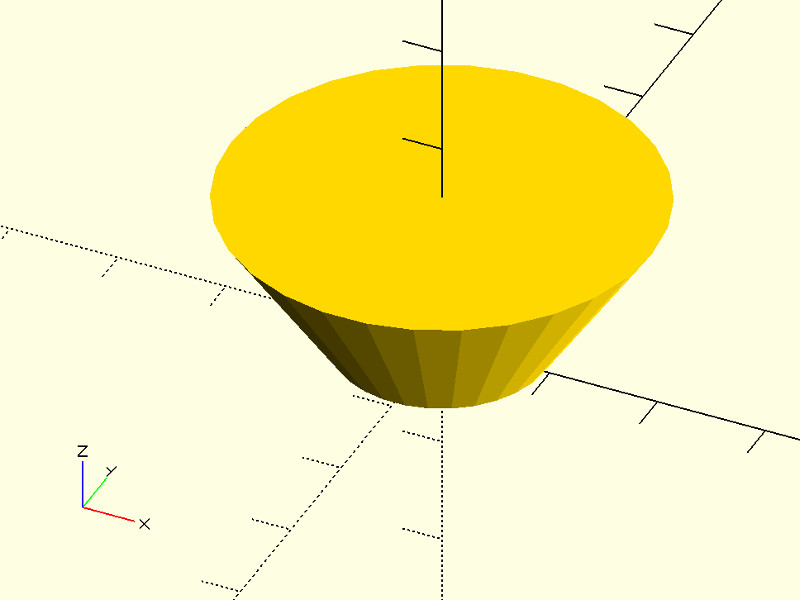
\includegraphics[width=7cm]{Img/Modelos/modelado5.jpg}
\centering
\caption{\textbf{a) \footnotesize{Un cilindro con radios diferentes. }}}
\end{figure}

\textbf{b)} Todos los scripts son equivalentes para este ejemplo:

\begin{minted}[baselinestretch=1]{python}
    cilindro(altura=15, r1=10, r2=0, centro=V)
    cilindro(15, 10, 0, V)
    cilindro(altura=15, d1=20, d2=0, centro=V)
\end{minted}

\begin{figure}[h]
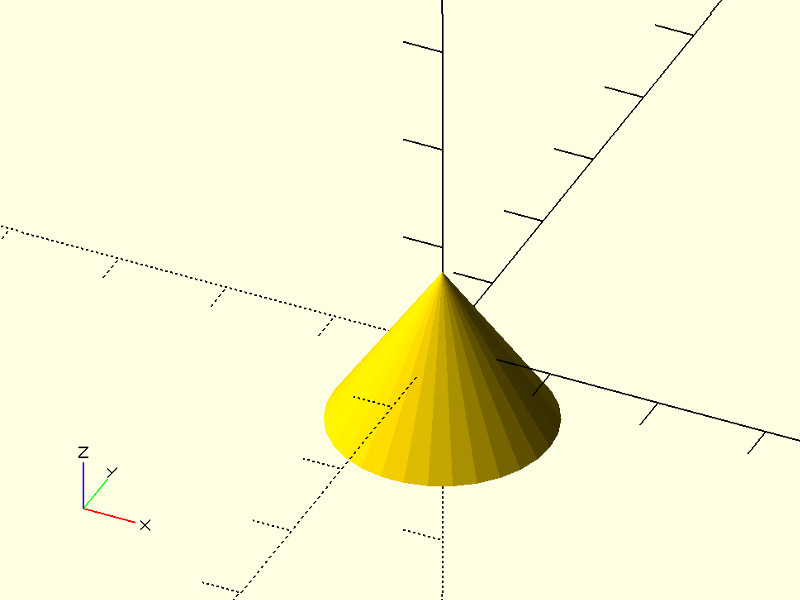
\includegraphics[width=7cm]{Img/Modelos/modelado6.jpg}
\centering
\caption{\textbf{b) \footnotesize{Un cono generado a partir de un cilindro.}}}
\end{figure}

Al aumentar los valores del parámetro \textbf{res} (resolución) se genera una superficie cada vez mas suave o lisa. A su vez, el uso de valores bajos de \textbf{res} produce algunos objetos no circulares que pueden ser útiles o interesantes. Algunos ejemplos a continuación:

\begin{minted}[baselinestretch=1]{python}
    cilindro(20, 20, 20, res=3)
    cilindro(20, 20,  0, res=4)
    cilindro(20, 20, 10, res=4)
\end{minted}

\begin{figure}[h]
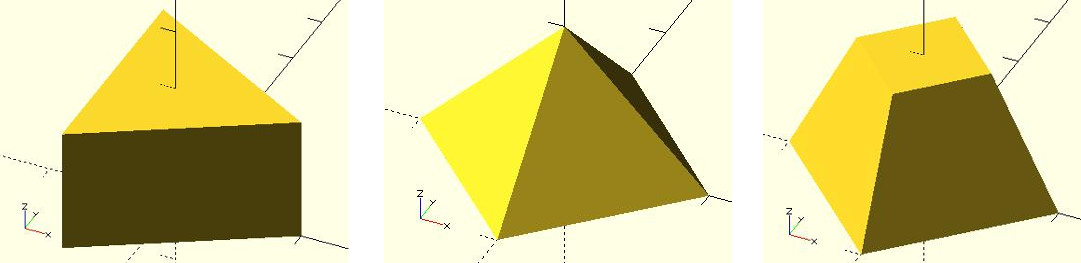
\includegraphics[width=12cm]{Img/Modelos/modelado7.jpg}
\centering
\caption{\textbf{b). \footnotesize{Figuras generadas a partir de un cilindro con baja resolución.}}}
\end{figure}

\clearpage
\subsubsection{Poliedro especificado en algoritmos}
El poliedro es una primitiva 3D genérica puede representar cualquier objeto sólido debido a que se define como un cuerpo geométrico cuyas caras son obligatoriamente planas y encierran un volumen como se vió en la sección \ref{sectionpoliedro}. A continuación vemos cómo especificar poliedros usando algoritmos.\vskip



\begin{description}
\item  \textbf{Parámetros:}
\item  \textbf{puntos}: Vector con puntos o vértices. Cada punto se define mediante un vector con sus coordenadas $[x,\ y,\ z]$.
Los puntos se pueden definir en cualquier orden. $N$ puntos son referenciados en un orden definido de $0$ a $N-1$.
\item  \textbf{caras}: Vector con caras que cierran la superficie del sólido. Cada cara es un vector que contiene los índices de 3 o más puntos pertenecientes al vector de puntos. 
Las caras se pueden definir en cualquier orden. Se debe definir suficientes caras para encerrar por completo el sólido, sin superposición entre ellas.
\end{description}

En el ejemplo \textbf{a)} se utiliza un poliedro para generar el mismo resultado que el siguiente cubo:

\begin{minted}{python}
    cubo([10, 7, 5])
\end{minted}

\begin{figure}[h]
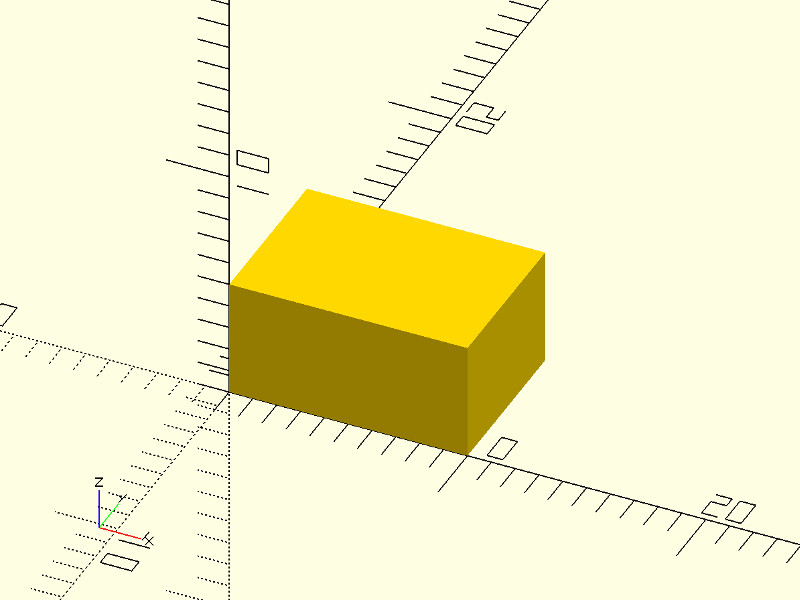
\includegraphics[width=8cm]{Img/Modelos/modelado9.jpg}
\centering
\caption{\textbf{\footnotesize{Resultado del algoritmo del poliedro para un cubo.}}}
\end{figure}

Para comprender como funciona el algoritmo \textbf{a)} del poliedro, observar la Figura \ref{fig:poliedrodes} que ilustra el despliegue del poliedro con sus vértices y caras.

\clearpage
\textbf{a)}
\begin{minted}[baselinestretch=1]{python}
    puntos = [ [ 0, 0, 0],  # 0
               [10, 0, 0],  # 1
               [10, 7, 0],  # 2
               [ 0, 7, 0],  # 3
               [ 0, 0, 5],  # 4
               [10, 0, 5],  # 5
               [10, 7, 5],  # 6
               [ 0, 7, 5] ] # 7
  
    caras = [ [0, 1, 2, 3],  # abajo
              [4, 5, 1, 0],  # frente
              [7, 6, 5, 4],  # arriba
              [5, 6, 2, 1],  # derecha
              [6, 7, 3, 2],  # atras
              [7, 4, 0, 3] ] # izquierda
  
    poliedro(puntos, caras)

\end{minted}

\begin{figure}[h]
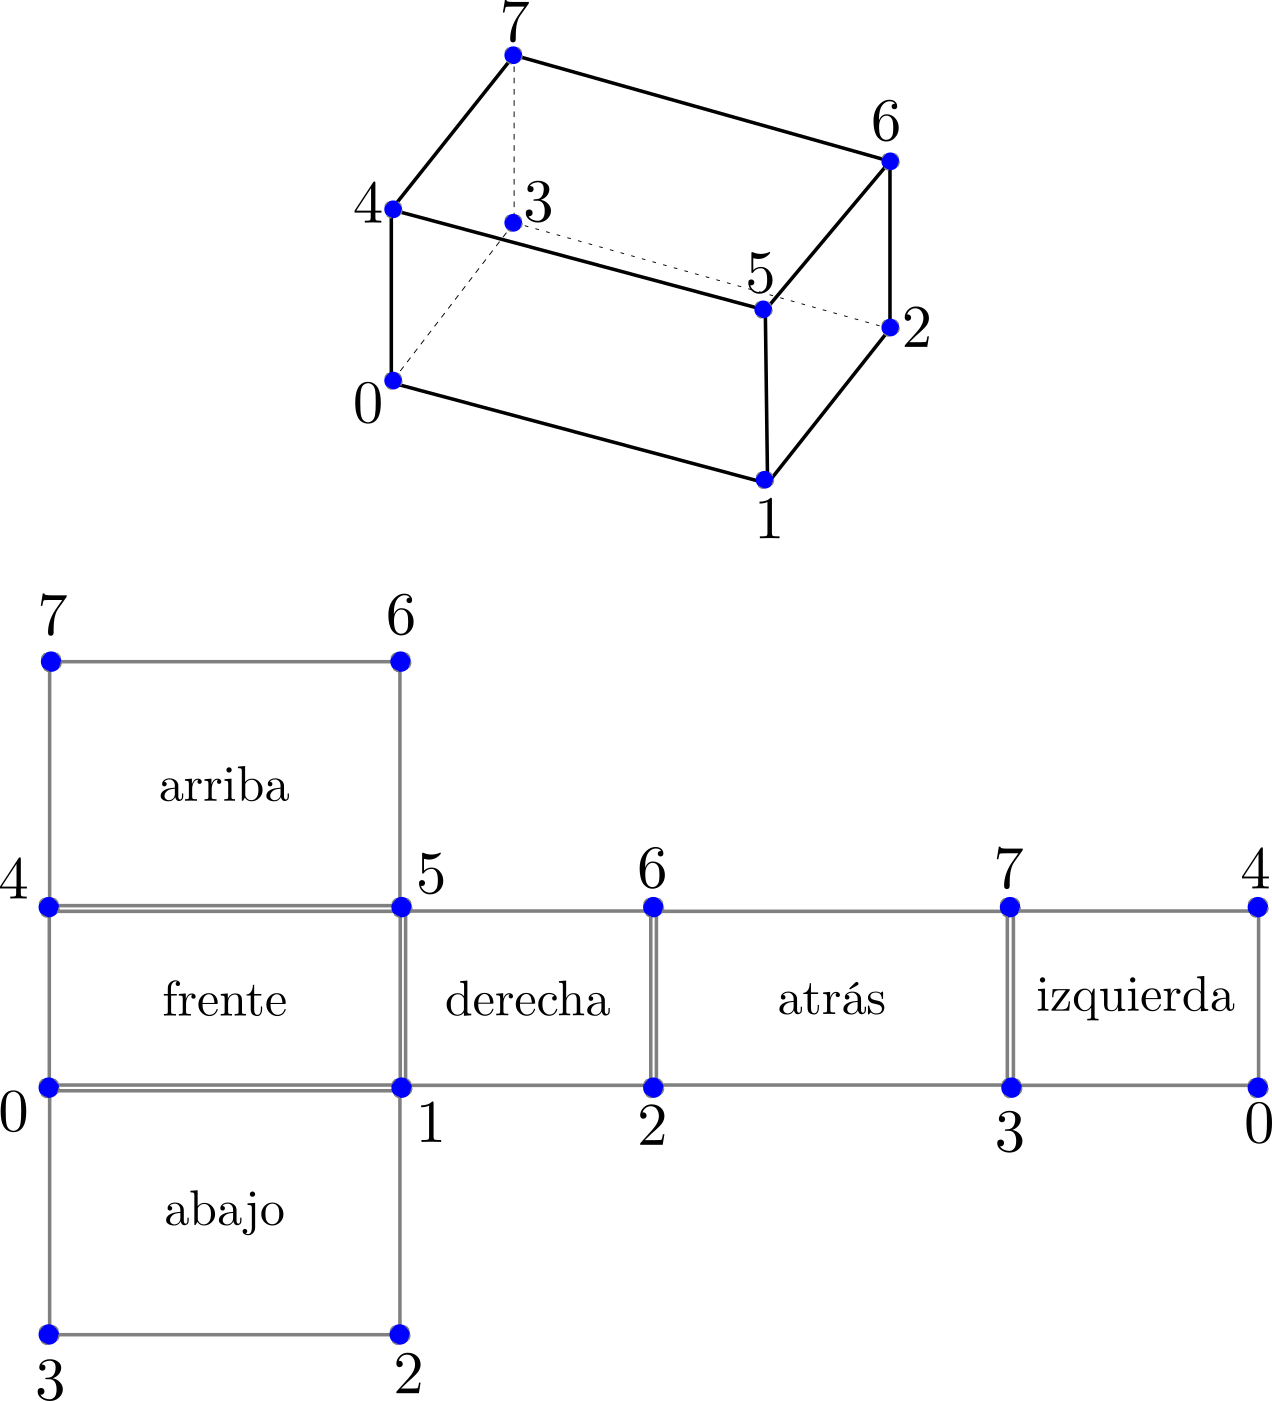
\includegraphics[width=10cm]{Img/Modelos/modelado8.png}
\centering
\caption{\textbf{ \footnotesize{Despliegue de poliedro con vértices y caras.}}}
\label{fig:poliedrodes}
\end{figure}

\clearpage
\textbf{b)} Una pirámide con base cuadrada

\begin{minted}[baselinestretch=1]{python}
    poliedro(
    puntos=[ [10, 10, 0], [10, -10, 0], [-10, -10, 0], [-10, 10, 0], 
          # los cuatro puntos de la base
           [0, 0, 10] ],  
          # la punta de la pirámide                                
    caras=[ [0, 1, 4], [1, 2, 4], [2, 3, 4], [3, 0 , 4],               
          # los triángulos de los lados
          [1, 0, 3], [2, 1, 3 ] ]                         
          # dos triángulos para la base cuadrada
    )

\end{minted}

\begin{figure}[h]
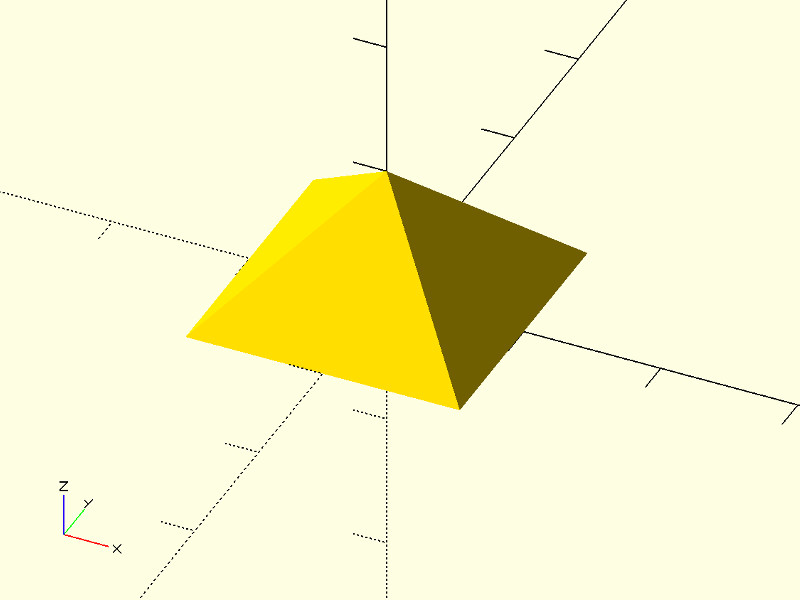
\includegraphics[width=8cm]{Img/Modelos/modelado10.jpg}
\centering
\caption{\textbf{ \footnotesize{Pirámide con base cuadrada.}}}
\end{figure}

\clearpage
Definir objetos mediante poliedros puede ser una herramienta muy potente, sin embargo su complejidad aumenta cuando se definen objetos con mucha resolución o con formas elaboradas. En el ejemplo \textbf{c)} se muestra un modelo de zapato generado a partir de \textbf{49818} triángulos. 

\textbf{c)} 

\begin{minted}[baselinestretch=1]{python}
    poliedro(
    puntos = [
        	[33.329444, 29.010915, 35.886886],
        	[30.592163, 29.074943, 29.971662],
        	[33.969806, 29.182254, 35.545883],
        	[30.592163, 29.074943, 29.971662],
        	... # A partir de esta linea 49814 vectores
        	]
    caras =  [
        	[0, 1, 2],
        	[3, 4, 5],
        	[6, 7, 8],
        	[9,10,11],
        	... # A partir de esta linea 49814 vectores
        	]
    )

\end{minted}

\begin{figure}[h]
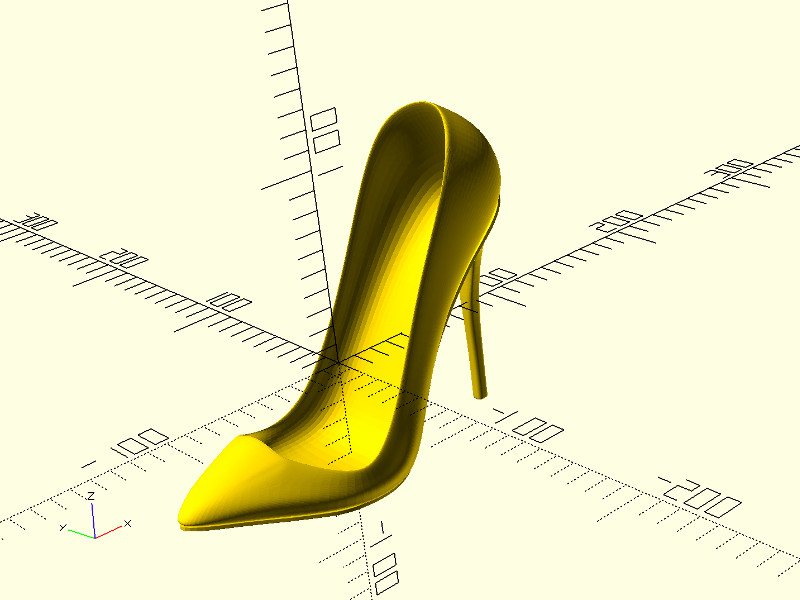
\includegraphics[width=8cm]{Img/Modelos/modelado14.jpg}
\centering
\caption{\textbf{ \footnotesize{Modelo de zapato formado por 49818 triángulos }}}
\end{figure}

\clearpage
\subsubsection{Transformaciones especificadas en algoritmos}

Las transformaciones se realizan mediante operadores indicando el objeto a transformar seguido de un $``."$ e indicando la acción a realizar (trasladar, escalar, rotar, etc). Las transformaciones compuestas se realizan utilizando el mismo mecanismo.

\begin{description}
\item  \textbf{Traslación - Parámetros:}
\item  \textbf{punto}: Vector con las coordenadas $[x,\ y, \ z]$ del punto al que se traslada el objeto.
\end{description}

\begin{minted}[baselinestretch=1]{python}
    a = cubo(10, centro=V)
    
    b = cubo(10, 10, 20)
    b.trasladar([15, 0, 0]) 
   
\end{minted}

\begin{figure}[h]
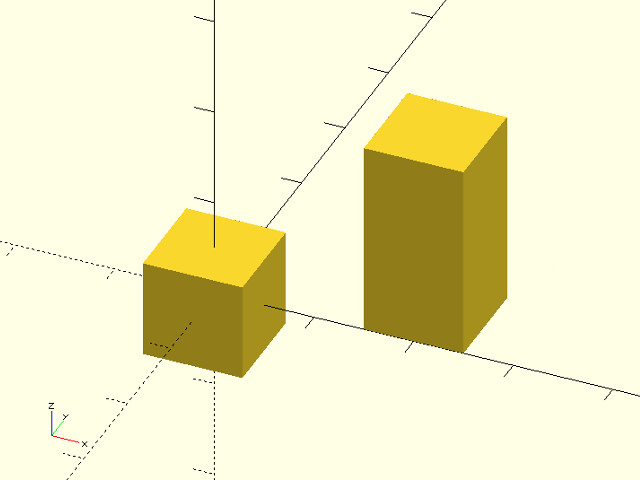
\includegraphics[width=8cm]{Img/Modelos/modelado11.jpg}
\centering
\caption{\textbf{ \footnotesize{Traslación del objeto $b$ (prisma rectangular) al punto $[15, 0, 0]$}}}
\label{fig:traslacion}
\end{figure}

\begin{description}
\item  \textbf{Escala - Parámetros:}
\item  \textbf{punto}: Vector con los factores de escalamiento en cada eje $[s_x,\ s_y, \ s_z]$.
\end{description}

\begin{minted}[baselinestretch=1]{python}
    a = cubo(10, centro=V)
    
    b = esfera(10, res=100).trasladar([0, 0, 30])
    b.escalar([0.5, 0.5, 2]) 
   
\end{minted}

\begin{figure}[h]
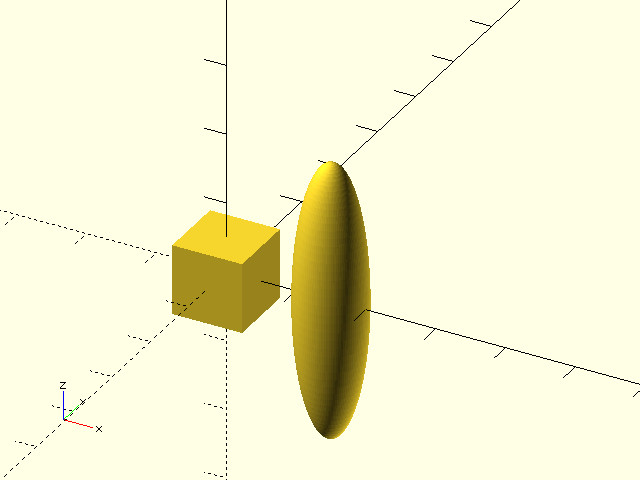
\includegraphics[width=8cm]{Img/Modelos/modelado12.jpg}
\centering
\caption{\textbf{ \footnotesize{Escala del objeto $b$ (esfera) por los factores de escalamiento $[0.5,\ 0.5,\ 2]$, el objeto es previamente trasladado al punto $[0,\ 0,\ 30]$ }}}
\end{figure}

\vskip
\begin{description}
\item  \textbf{Rotacion - Parámetros:}
\item  \textbf{punto}: Vector con los ángulos de rotación del objeto sobre los ejes coordenados $[x,\ y, \ z]$ especificados en grados $^\circ$.
\end{description}


\begin{minted}[baselinestretch=1]{python}
    a = cubo([5, 10, 20]).trasladar([20,0,0])
    a.rotar([45,0,0]) # Rotar 45 º sobre el eje X

    b = cubo([5, 10, 20]).trasladar([20,0,0])
    b.rotar([0,-45,0]) # Rotar -45 º sobre el eje Y

    c = cubo([5, 10, 20]).trasladar([-20,0,0])
    b.rotar([0,0,45]) # Rotar 45 º sobre el eje Z

\end{minted}

\begin{figure}[h]
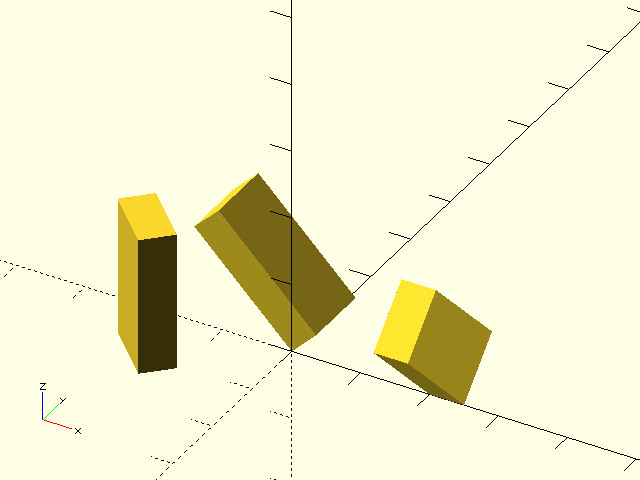
\includegraphics[width=8cm]{Img/Modelos/modelado13.jpg}
\centering
\caption{\textbf{ \footnotesize{Rotación de 3 objetos sobre los tres ejes coordenados. }}}
\end{figure}

\clearpage
\subsubsection{Operaciones booleanas especificadas en algoritmos}
Las operaciones booleanas se realizan mediante operadores indicando el objeto a aplicar seguido de un “.” y la acción a realizar (intercectar, unir, substraer), como parámetro se indica el otro objeto. ej. \textbf{objeto1.unir(objeto2)}
\vspace{5mm}

\textbf{a)} Operaciones booleanas de los objetos \textbf{a} (cubo) y \textbf{b} (esfera). Ver Figura \ref{aCSG} \vskip

Los objetos solidos $a$ y $b$ son generados con el siguiente código  

\begin{minted}[baselinestretch=1]{python}
    a = cubo(100)
    b = esfera(65).trasladar([65, 65, 65])
\end{minted}

Operaciones booleanas simples:

\begin{minted}[baselinestretch=1, bgcolor=LightGray]{python}
    a.unir(b)
    # Sentencias equivalentes
    cubo(100).unir( esfera(65).trasladar([65, 65, 65]) )
\end{minted}

\begin{minted}[baselinestretch=1, bgcolor=LightGray]{python}
    a.substraer(b)
    # Sentencias equivalentes
    cubo(100).substraer( esfera(65).trasladar([65, 65, 65]) )
\end{minted}

\begin{minted}[baselinestretch=1, bgcolor=LightGray]{python}
    a.intersectar(b)
    # Sentencias equivalentes
    cubo(100).intersectar( esfera(65).trasladar([65, 65, 65]) )
\end{minted}

\textbf{b)} En este ejemplo se construye un sólido mediante operaciones booleanas combinadas como se analiza en la sección \ref{sectionCSG}. Ver Figura \ref{bCSG} \vskip

Los objetos solidos \textbf{a}, \textbf{b}, \textbf{c}, \textbf{d} y \textbf{e} son generados con el siguiente código  


\begin{minted}[baselinestretch=1, bgcolor=LightGray]{python}
    a = cubo(100, centro=V)
    b = esfera(65)
    c = cilindro(longitud=130, r=32.5, centro=V).rotar([90, 0, 0])
    d = cilindro(longitud=130, r=32.5, centro=V)
    e = cilindro(longitud=130, r=32.5, centro=V).rotar([0, 90, 0])
\end{minted}

Operaciones booleanas combinadas:

\begin{minted}[baselinestretch=1, bgcolor=LightGray]{python}
    a.intersectar(b).substraer(c.unir(d).unir(e))
\end{minted}

\begin{figure}[h]
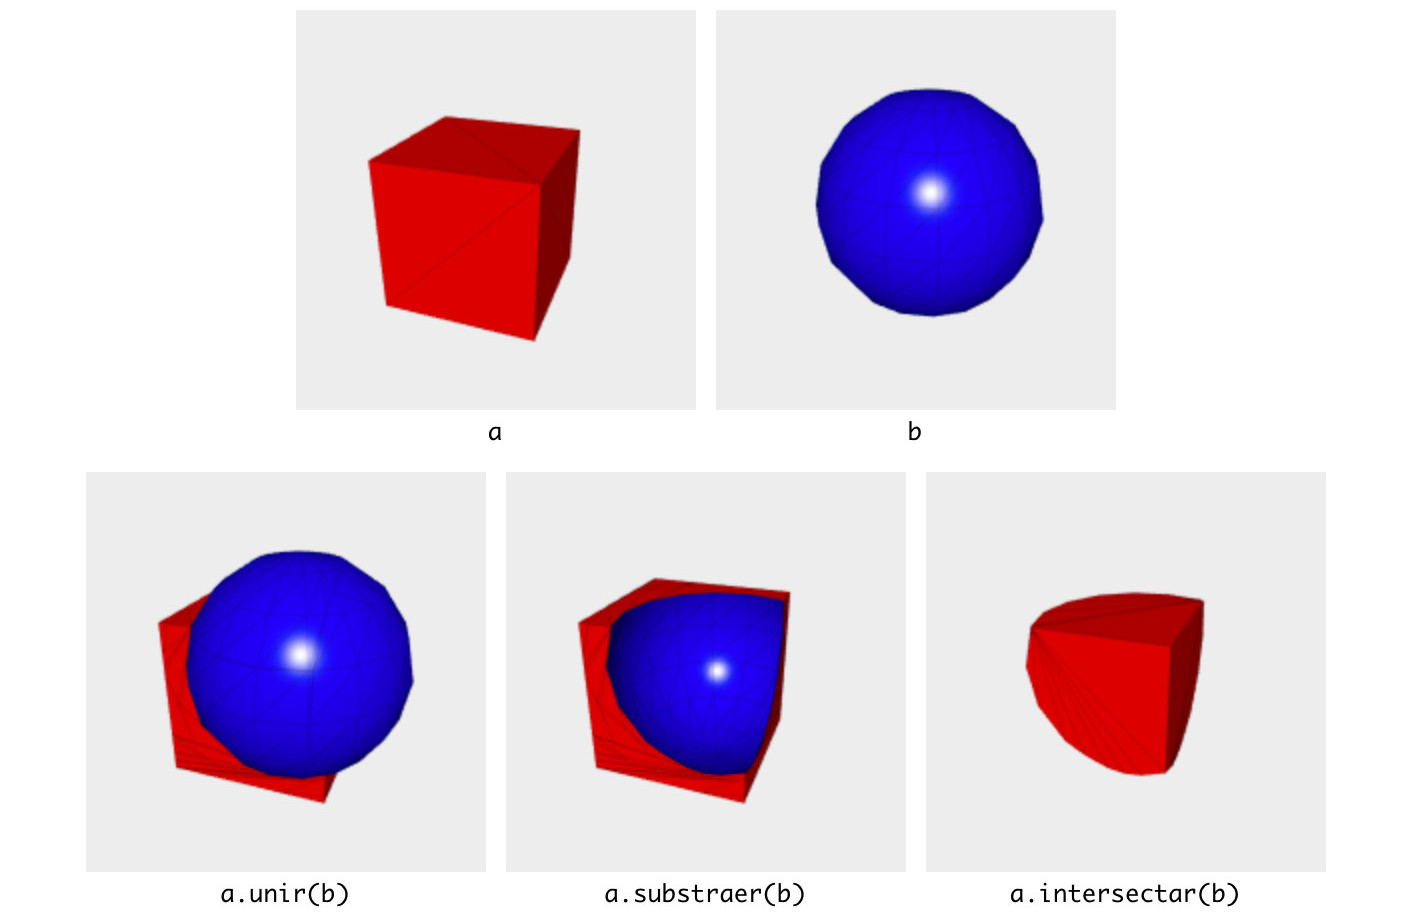
\includegraphics[width=14cm]{Img/Modelos/modelado15.jpg}
\centering
\caption{\textbf{ \footnotesize{a) Operaciones booleanas simples }}}
\label{aCSG}
\end{figure}


\begin{figure}[h]
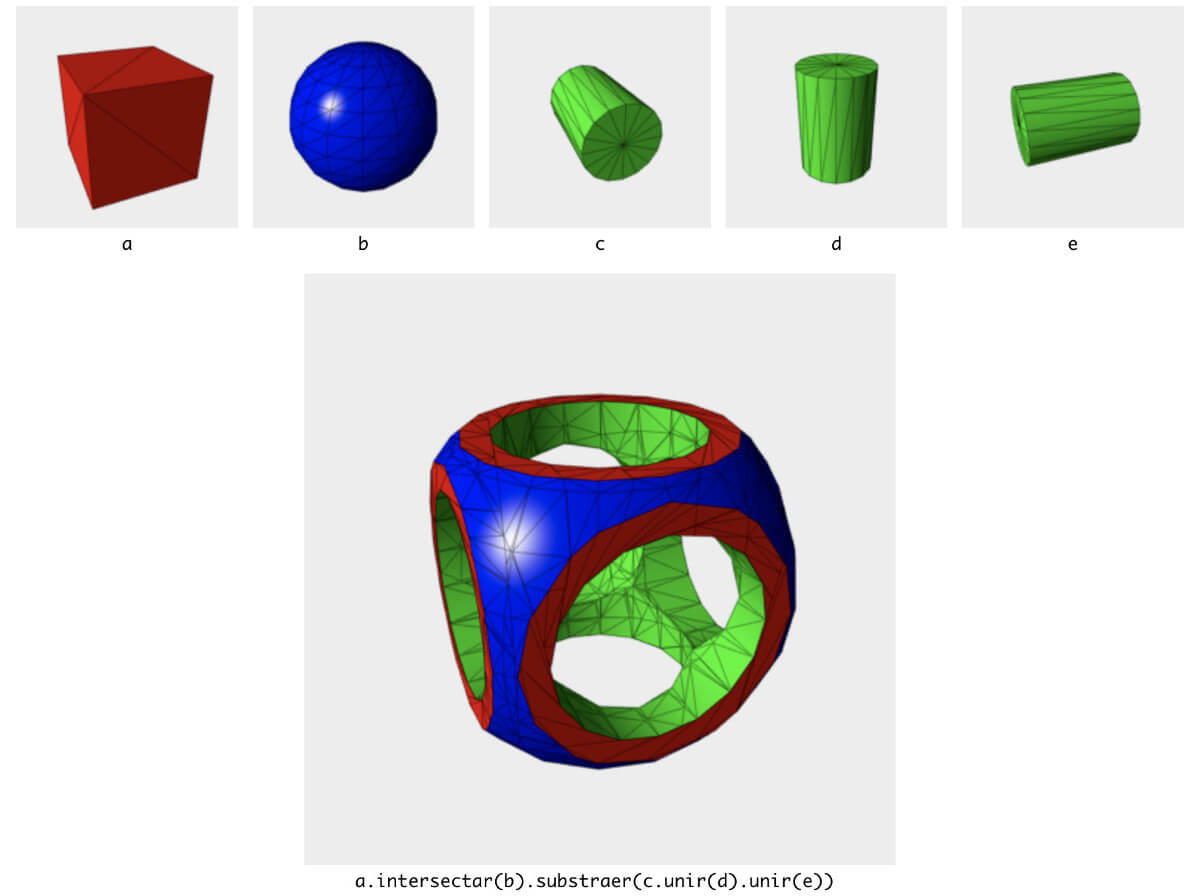
\includegraphics[width=16cm]{Img/Modelos/modelado16a.jpg}
\centering
\caption{\textbf{ \footnotesize{b) Operaciones booleanas combinadas }}}
\label{bCSG}
\end{figure}
\clearpage

\subsubsection{Polígonos (2D) especificados en algoritmos}
Los polígonos no son sólidos geométricos, sin embargo pueden ser utilizados como base para la construcción de modelos 3D sólidos. Los polígonos también pueden manipularse utilizando transformaciones.

\begin{description}
\item  \textbf{Cuadrado - Parámetros:}
\item   \textbf{longitud}:
\begin{description}
\item \textbf{1 valor} único que especifica la longitud de todos los lados del cuadrado.
\item \textbf{2 valores} especificando dimensiones $x$, $y$.
\end{description}
\item   \textbf{centro}:
\begin{description}
\item \textbf{F} Falso (por defecto), 1er cuadrante positivo, esquina en $(0, 0)$
\item \textbf{V} Verdadero, el centro del cuadrado está en $(0, 0)$
\end{description}
\end{description}

\textbf{a) Cuadrado y rectángulo} 

\begin{listing}[ht]
\begin{minted}[baselinestretch=1]{python}
    a = cuadrado(20, 20, centro = V)
    
    b = cuadrado(40, 20, centro = V).trasladar( [50, 0, 0] ) 
    # Rectángulo
\end{minted}
\end{listing}

\begin{figure}[h]
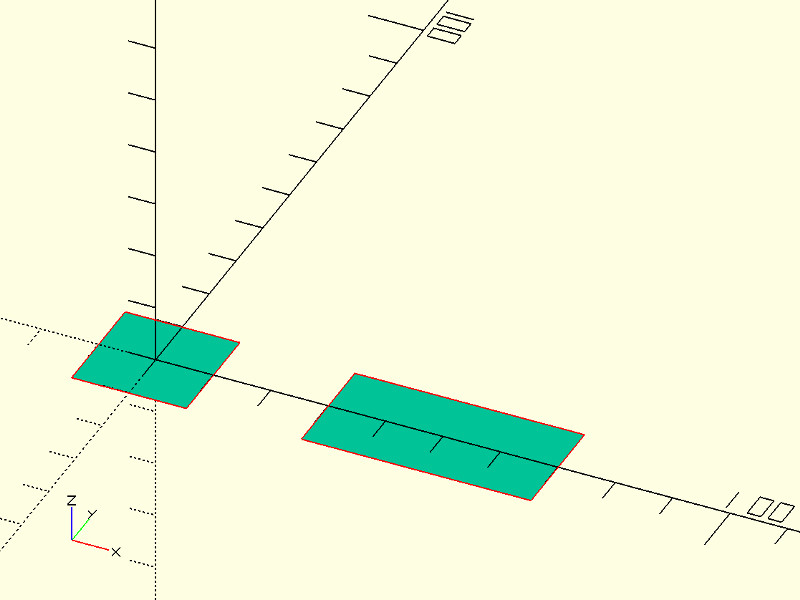
\includegraphics[width=8cm]{Img/Modelos/modelado17.jpg}
\centering
\caption{\textbf{ \footnotesize{a) a=cuadrado y b=rectángulo}}}
\end{figure}

\clearpage
\begin{description}
\item \textbf{Círculo - Parámetros:}
\item  \textbf{r}: Radio del círculo.
\item  \textbf{d}: Diámetro del círculo.
\item  \textbf{res}: Resolución del círculo.
\end{description}

\textbf{a)} 
\begin{listing}[ht]
\begin{minted}[baselinestretch=1]{python}
    a = circulo(r=20, res=3).trasladar( [-50, 0, 0] )
    b = circulo(r=20, res=4).trasladar( [ 0, 0, 0] )
    c = circulo(r=20, res=5).trasladar( [50, 0, 0] )
    d = circulo(r=20, res=6).trasladar( [-50, -50, 0] )
    e = circulo(r=20, res=8).trasladar( [ 0, -50, 0] )
    f = circulo(r=20, res=50).trasladar( [ 50, -50, 0] )
\end{minted}
\end{listing}

\begin{figure}[h]
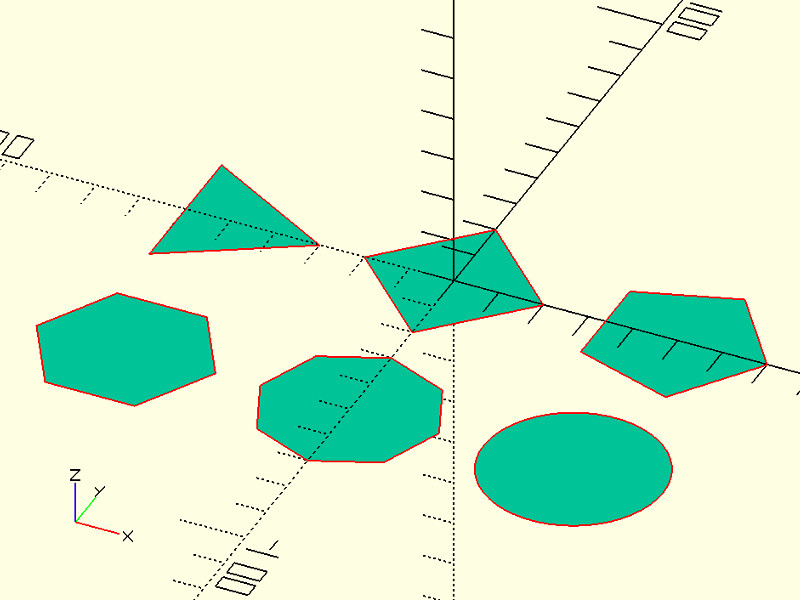
\includegraphics[width=8cm]{Img/Modelos/modelado18.jpg}
\centering
\caption{\textbf{\footnotesize{a) círculos con diferentes resoluciones que producen diferentes polígonos a=triangulo, b=cuadrado, c=pentágono, d=hexágono, e=heptágono y f=círculo  }}}
\end{figure}


\clearpage
\subsubsection{Operaciones de barrido especificadas en algoritmos}

El barrido translacional o \textbf{extrusión} es una operación de modelado que parte de un polígono (cuadrado, rectángulo, circulo) y lo extiende a la tercera dimensión (sólido 3D). Para simplificar el funcionamiento se considera que el modelo parte del plano \textit{xy} hasta una longitud indicada en el plano \textit{z}. Es posible aplicar otras transformaciones combinadas con la extrusión.

\begin{description}
\item  \textbf{Extrusión - Parámetros:}
\item  \textbf{longitud}: Longitud de la extrusión (debe ser positivo).
\item  \textbf{torsion}: Rotación en  ángulos $^\circ$ sobre el eje \textbf{z}.
\end{description}

\textbf{a) Extrusión de polígonos} 


\begin{listing}[ht]
\begin{minted}[baselinestretch=1]{python}
    a = circulo(r=5).trasladar( [10, 0, 0] )
    a.extruir(100, torsion = -500)
    
    b = circulo(r=10, res=5).trasladar( [50, 0, 0] )
    b.extruir(100, torsion = 0)
    
    c = cuadrado(20).trasladar( [100, 0, 0] ).escalar( [1, 0.1, 1] )
    c.extruir(longitud = 100,  torsion = 0)
\end{minted}
\end{listing}

\begin{figure}[h]
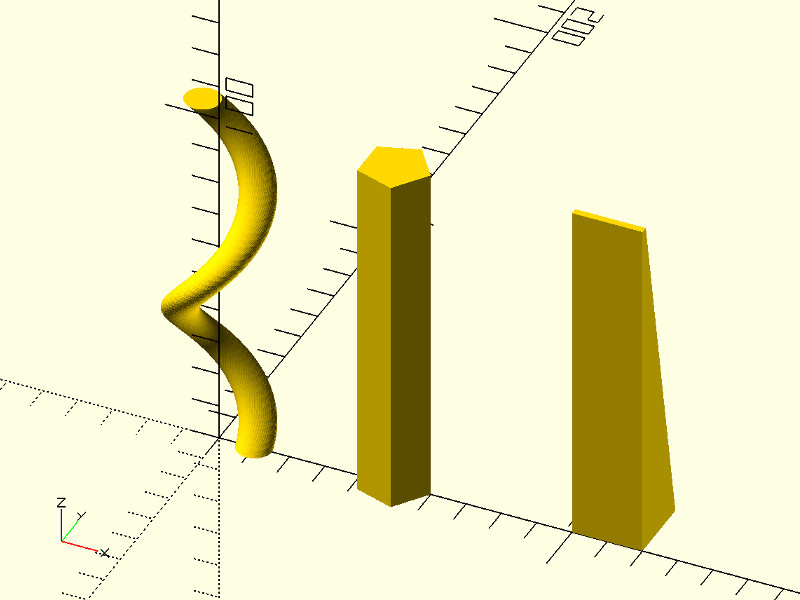
\includegraphics[width=8cm]{Img/Modelos/modelado19.jpg}
\centering
\caption{\textbf{\footnotesize{a) a=círculo convertido en un cilindro con torsion de $-500^\circ$, b=pentágono convertido en un prisma, c=cuadrado convertido en un poliedro de base rectangular.}}}
\end{figure}


\clearpage


\subsection{Modelos 3D en la web.}

Las aplicaciones web están ingresando rápidamente en dominios donde las aplicaciones de escritorio fueron la única alternativa viable. Desde la perspectiva de los desarrolladores, es muy interesante por qué ha aumentado el interés en estas aplicaciones basadas en el navegador web. Las aplicaciones resultantes se pueden ejecutar con cualquier combinación de hardware y sistema operativo que permita el uso de un navegador web moderno, incluidos dispositivos como teléfonos móviles y tabletas. Además, el usuario final no tiene que instalar el software en su dispositivo para usarlo, esto se realiza automáticamente mediante el navegador web y cualquier complemento asociado. En general, las aplicaciones web ofrecen a los desarrolladores la oportunidad de llegar a una gran audiencia sin muchas dificultades para dar soporte a múltiples plataformas, como sucedía anteriormente con las aplicaciones de escritorio. \vskip

Incluir gráficos 3D en aplicaciones web no es una nueva tendencia. En 1994, se estandarizó una forma de presentar escenas 3D en el navegador web a través de un lenguaje de marcado llamado VRML. VRML permite que las escenas 3D se especifiquen en un lenguaje similar al HTML. Si bien hay (o ha habido) aplicaciones de nicho que usan VRML, hoy en día existen pocos sitios populares que incluyen documentos VRML. Parece haberse convertido en un estándar que nunca creció lo suficientemente ni se utilizo demasiado como para ver un uso significativo a gran escala. Es probable que el motivo fué la potencia de procesamiento disponible, sobre todo en computadoras de precios razonables, que en esa época no fueron lo suficientemente potentes para proporcionar gráficos 3D convincentes. Esto ha cambiado recientemente con procesadores gráficos dedicados que se abren paso en más y más tipos de dispositivos. Gracias a esto, ha habido un renovado interés en las tecnologías que proporcionan gráficos 3D en páginas web y en aplicaciones web.\vskip

Los gráficos 3D interactivos son una de las áreas más grandes e importantes donde las aplicaciones web no tuvieron mucho éxito hasta hace poco. Parte de esto se debe a que este tipo de interactividad exige comprometer en gran parte del dispositivo y el software relacionado, como las máquinas virtuales para lenguajes de scripting tan a menudo involucradas en este tipo de aplicaciones. Otra razón fué la falta de una Interfaz de Programación de Aplicaciones en inglés  Application Programming Interface (API) para gráficas 3D en la mayoría de las tecnologías de aplicaciones web. Ambas áreas han visto mejoras, la primera con técnicas tales como compilación just-in-time (JIT)\footnote{Un compilador JIT (Just-In-Time) es un componente de software que mejora el rendimiento de las aplicaciones compilando códigos de bytes en código de máquina nativa, en tiempo de ejecución. } y la segunda con la introducción de tecnologías como Stage 3D para Flash\footnote{\url{https://www.adobe.com/devnet/flashplayer/stage3d.html}} y WebGL. \citep{Waerner2012}  
\vskip

La realidad de las aplicaciones actuales implica que las soluciones sean capaces de ejecutarse en más plataformas, admitir más navegadores y dispositivos, por lo tanto, se vuelve fundamental elegir una tecnología desde una perspectiva de compatibilidad, como WebGL. La Figura \ref{fig:compa} muestra la compatibilidad de WebGL con los navegadores más utilizados y sus respectivas versiones.

\begin{figure}[h]
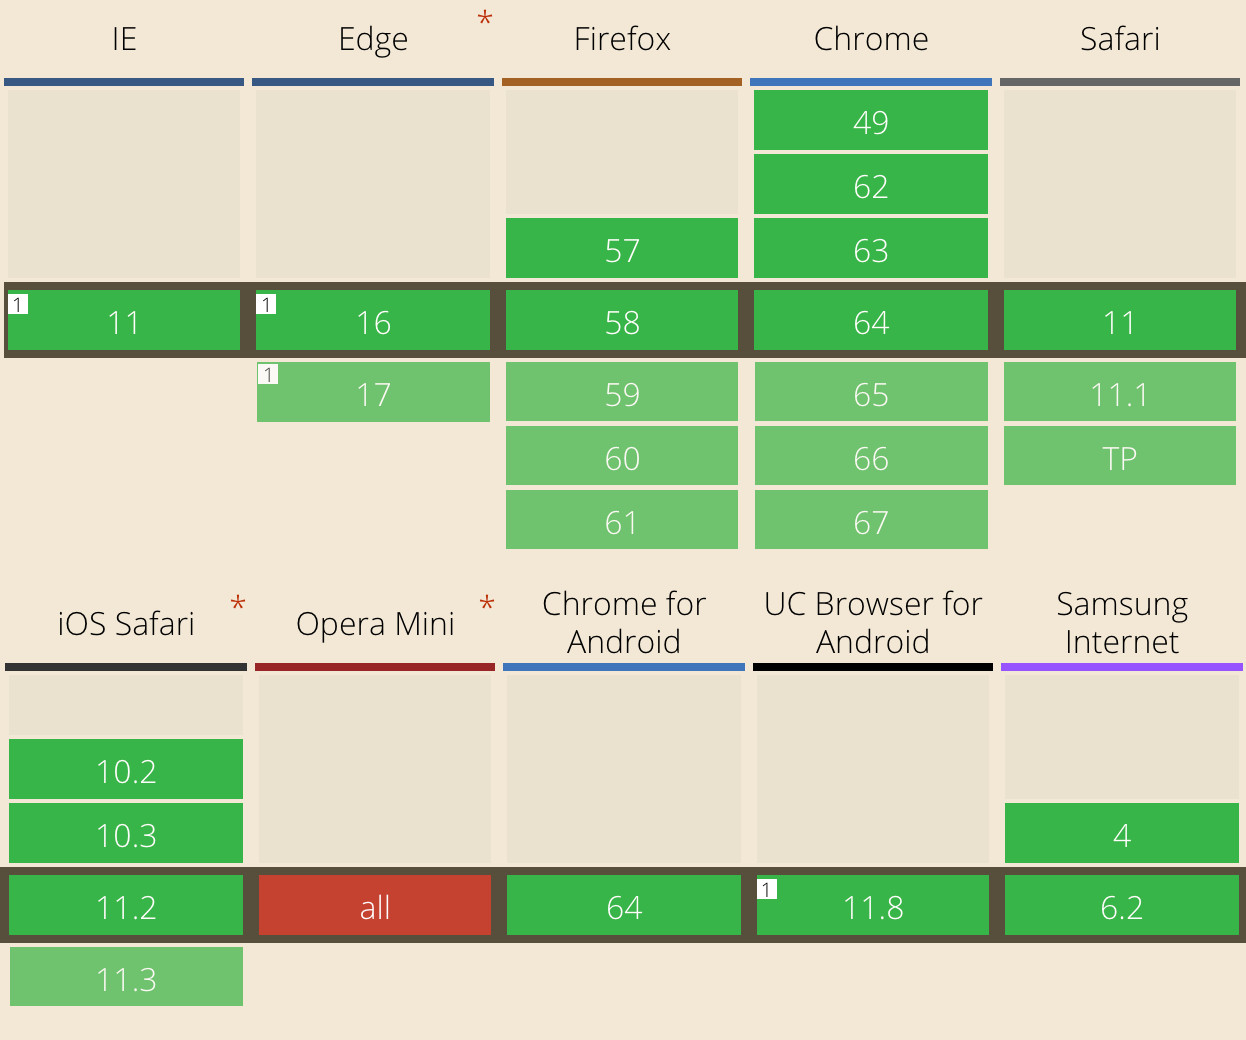
\includegraphics[width=16cm]{Img/WEB/web-compa.jpg}
\centering
\caption{\textbf{\footnotesize{Compatibilidad de WebGL con navegadores web. Verde (Soportado) y Rojo (No soportado). Fuente \url{https://caniuse.com/#feat=webgl} }}}
\label{fig:compa}
\end{figure}


\subsubsection{WebGL}

WebGL\footnote{\url{https://www.khronos.org/webgl/}} en inglés \textit{Web Graphic Library} es una API de JavaScript que permite implementar gráficos 3D interactivos directamente en el navegador. Fué desarrollado por la fundación Mozilla en 2006, con la intención de proporcionar una API de gráficos 3D para el elemento canvas\footnote{\url{https://developer.mozilla.org/es/docs/Web/HTML/Canvas}} de HTML. El diseño se basó en OpenGL ES 2.0, que es un subconjunto de OpenGL destinado a sistemas embebidos. La especificación WebGL es mantenida desde el 2009 por Khronos Group. No es parte de la especificación HTML5 oficial, pero en la actualidad es compatible con todos los principales navegadores y se ha convertido en la API estándar para gráficos 3D en navegadores. \vskip 


``Bajo nivel" significa que los comandos WebGL se expresan en términos que se relacionan de manera relativamente directa a cómo funciona realmente una GPU (unidad de procesamiento de gráficos, es decir, hardware). Eso significa que WebGL permite aprovechar realmente el conjunto de características y la potencia del hardware de gráficos. De la misma manera que los juegos nativos hacen con OpenGL o Direct3D, probablemente también lo pueden hacer con WebGL. \citep{Nyman2013}

WebGL es de tan bajo nivel que ni siquiera es una API de gráficos ``3D", definiéndola correctamente. Al igual que para el hardware de gráficos es indistinto si está procesando gráficos 2D o 3D. En WebGL, 2D y 3D son solo dos posibles patrones de uso.\vskip Cuando OpenGL 1.0 salió en 1992, era específicamente una API 3D, con el objetivo de exponer las características del hardware de gráficos 3D de esa época, a medida que éste fué evolucionando para ser más genérico y programable, también lo hizo OpenGL. Eventualmente, OpenGL se volvió tan genérico que el 2D y 3D son solo dos casos de uso posibles, a la vez que ofrecen un gran rendimiento. Ese fué el caso de OpenGL 2.0, y WebGL siguió ese concepto en su desarrollo.

A eso se refiere la definición de WebGL como una API de gráficos de bajo nivel en lugar de una API 3D específica. 

Sin embargo, la naturaleza genérica de WebGL hace que desarrollar en contextos de gráfica sea una tarea engorrosa como se puede apreciar en la documentación de la API y tutoriales de la comunidad \citep{MozillaFoundation}. Para solventar este hecho, se construyeron frameworks y librerías con WebGL como base para proporcionar una interfaz de más alto nivel para la API. Las opciones de software para desarrollar gráficas en la web son muy variadas, desde representación de gráficos vectoriales escalables en inglés Scalable Vector Graphics (SVG)\footnote{\url{https://www.w3.org/Graphics/SVG/}} hasta realidad virtual con WebVR\footnote{\url{https://webvr.info/}}. A continuación se analizan y evalúan dos de estas tecnologías, que se consideran técnicamente aptas para cumplir con los objetivos de este trabajo.

\subsubsection{OpenJSCAD}

OpenJSCad\footnote{\url{https://openjscad.org/}}
es un conjunto de herramientas modulares para diseño paramétrico 2D y 3D, que pueden ejecutarse en el navegador web y a través de interfaces de linea de comandos mediante código JavaScript. A continuación algunas características:

\begin{itemize}
    \item Se puede ejecutar en el navegador web sin necesidad instalar ningún software extra.
    \item Se puede instalar todas las capacidades de la web oficial del proyecto en un servidor propio.
    \item Posee una Interfaz de linea de comandos en ingles \textit{Command Line Interface} (CLI) para computar los modelos en el servidor con Node.js.
    \item Se visualiza en el navegador mediante webGL, haciendo uso de canvas de HTML5.
    \item Soporta modelos paramétricos con parámetros editables por el usuario sin la necesidad de editar el script de origen.
    \item Soporta modelado booleano CSG y transformaciones geométricas.
    \item Los sólidos se almacenan en variables. Esto permite, permite operaciones como la clonación de objetos.
    \item Amplio soporte para matemáticas 2D y 3D (clases para Vector2D, Vector3D, Plane, Line3D, Line2D).
    \item Los sólidos 3D se puede exportar a archivos STL, las áreas 2D se pueden exportar con archivos DXF. También permite la importación en ambos casos.
\end{itemize}

\subsubsection{Creación de un cubo con OpenJSCAD}

Un script OpenJSCAD debe tener al menos una función definida, la funcion $main()$, que retorna un objeto CSG o un vector (array) de dos o más objetos CSG. En el siguiente ejemplo se crea un cubo azul con código OpenJSCAD, se puede ver el resultado en la Figura \ref{fig:jopen}. 

\begin{minted}[baselinestretch=1, bgcolor=LightGray, linenos]{js}
 function main() {
     // Cubo de tamaño 20 de color azul
     return cube({size: 20}).setColor([0, 0, 1]);
 }
\end{minted}

\begin{figure}[h]
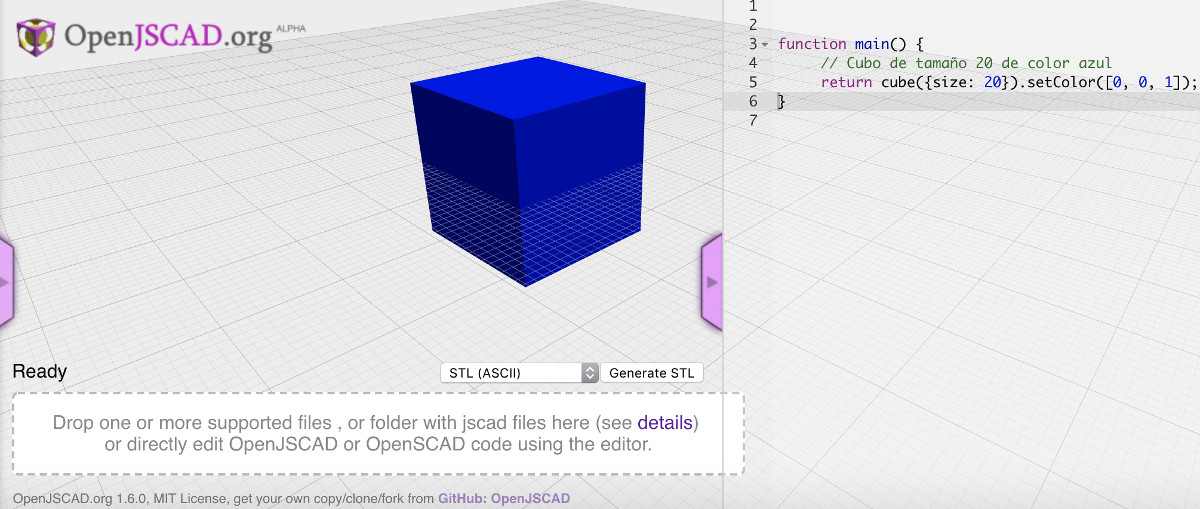
\includegraphics[width=15cm]{Img/WEB/web-jopen.jpg}
\centering
\caption{\textbf{\footnotesize{Interfaz de OpenJSCAD }}}
\label{fig:jopen}
\end{figure}


Para trabajar con modelado booleano OpenJSCAD utiliza una librería llamada CSG.js \footnote{\url{https://github.com/jscad/csg.js}}, esta librería implementa operaiones CSG mediante BSP trees. Para la visualiación utiliza lightgl.js \footnote{\url{https://github.com/evanw/lightgl.js/}} que facilita el prototipado rápido de aplicaciones WebGL implementando funciones de Ray Tracing, funciona a un nivel más bajo que muchas otras bibliotecas WebGL y aunque no proporciona un esquema de escena, implementa un mecanismo modelo-vista/proyección\footnote{\url{http://www.opengl-tutorial.org/es/beginners-tutorials/tutorial-3-matrices/}} similar a OpenGL.

\subsubsection{Three.js
}

Three.js\footnote{\url{https://threejs.org/}} es una librería/API desarrollada en JavaScript y soportada en la mayoría de los navegadores web. Es utilizada sobre todo para crear y visualizar gráficos 3D animados en los navegadores web. Los scripts de Three.js se pueden utilizar mediante canvas de HTML5, SVG o WebGL. Contiene abstracciones de alto nivel para tareas comunes de WebGL y proporciona, entre otras capacidades, las siguientes:

\begin{itemize}
    \item Se puede ejecutar en el navegador web sin necesidad instalar ningún software extra.
    \item Se puede instalar utilizando NPM y Node.js.
    \item Capacidad de gestionar objetos en un escena.
    \item Render usando WebGL, SVG o incluso CSS (con el propósito de soportar navegadores sin soporte de WebGL).
    \item Matemáticas relacionadas con 3D, marcadores de fronteras, transformaciones en objetos de la escena.
    \item Trabajar con una gran cantidad de objetos predefinidos como Primitivas, Materiales (shaders), Luces, Cámaras.
    \item Efectos gráficos como desenfoque de cámara.
    \item Cargadores para archivos de modelos 3D como Collada, STL, Obj.
    \item Puede trabajar con audio mediante WebAudio API\footnote{\url{https://developer.mozilla.org/es/docs/Web_Audio_API}}.
    \item Animación por keyframes usando esqueletos y otros sistemas.
    \item Simulaciones físicas como colisiones, telas, iluminación realista.
\end{itemize} 

\subsubsection{Creación de un cubo con Three.js}

Para poder mostrar algo realmente  con three.js, se necesitan tres cosas: \textit{escena, cámara y renderizador}. Esto es obligatorio para poder renderizar la escena mediante la cámara. En el siguiente ejemplo se crea un cubo azul con código Three.js. 

\begin{minted}[baselinestretch=1, bgcolor=LightGray, linenos]{js} 

 // Se crea una escena
 scene = new THREE.Scene();

 // Se crea una cámara
 camera = new THREE.PerspectiveCamera();
 camera.position.x = 0;
 camera.position.y = 0;
 camera.position.z = 60;
	
 // Se agrega la cámara a la escena		
 scene.add( camera );

 // Se crea un material de color azul			
 var material= new THREE.MeshBasicMaterial( { color: 0x0000ff } );
 // Se crea un cubo de tamaño 20, con el material de color azul 
 cube = new THREE.Mesh( new THREE.CubeGeometry( 20, 20, 20 ), 
 material );
 // Se agrega el cubo a la escena
 scene.add( cube );


 // Se crea un renderizador
 renderer = new THREE.CanvasRenderer();

 // Se realiza el render de la escena con la cámara
 renderer.render( scene, camera );

\end{minted}

Three.js utiliza el concepto de gráfico de escena en inglés \textit{Scene Graph}. La mayoría de los motores 3D usan este concepto, se colocan los objetos que se necesitan visualizar en el gráfico de escena. El motor recorre el gráfico de la escena y calcula una lista de elementos para dibujar. Un gráfico de escena es una colección de nodos en estructura de árbol jerárquico.

Una escena es un soporte para todos los objetos que componen un mundo en 3D, incluidas las luces, los objetos gráficos y posiblemente las cámaras. Actúa como un nodo raíz para el gráfico de escena. Una cámara es un tipo especial de objeto que representa un punto de vista desde el cual se puede hacer una imagen de un mundo 3D. Representa una combinación de una transformación de visualización y una proyección. Un procesador es un objeto que crea la imagen. Los renderizadores siempre dibujarán la imagen en un canvas de HTML.

\begin{figure}[h]
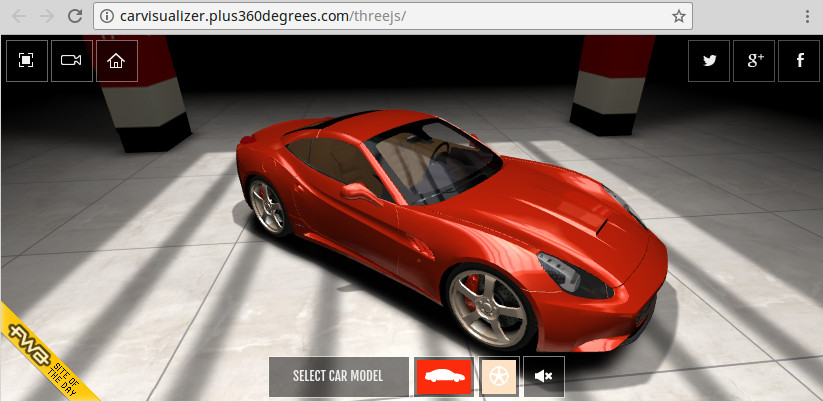
\includegraphics[width=15cm]{Img/WEB/web-three.jpg}
\centering
\caption{\textbf{\footnotesize{Ejemplo de aplicación con Three.js fuente: \url{http://carvisualizer.plus360degrees.com/threejs/} }}}
\label{fig:threejs}
\end{figure}

\clearpage
\subsubsection{Evaluación}

A continuación en la tabla se analizan las OpenJSCAD y Three.js respecto a los requerimientos del prototipo COCADA.

\begin{center}
 \begin{tabular}{ c |c c } 
   \empty & OpenJSCAD & Three.js  \\ 
   \hline
   Enfoque de modelado booleano CSG & Sí & No \\
   \hline
   Visualizacion vía WebGL & Sí & Sí \\
   \hline
   Implementación de Ray Tracing & Sí & Sí \\
   \hline
   Interfaz CLI & Sí & No \\
   \hline
   Compatibilidad con la mayoría de los navegadores & Sí & Sí \\
   \hline
   Importación/Exportación de otros formatos & Sí & Sí \\
   \hline
   
   
\end{tabular}
\end{center}
\vskip
\begin{center}
\caption{Tabla comparativa entre OpenJSCAD y Three.js}
\end{center}

Si bien las funcionalidades de ambas tecnologías pueden ser similares, es importante aclarar el ámbito de aplicación de cada una respecto al prototipo.

\begin{itemize}
    \item OpenJSCAD es un conjunto de herramientas que permiten resolver el modelado mediante scripting en la web, con una calidad de visualización suficiente para poder comprender la geometría de un modelo sólido.
    \item Three.js es una librería que puede realizar modelado booleano mediante complementos o plugins\footnote{Los complementos o plugins son herramientas que extienden la funcionalidad de un software}, sin embargo se utiliza normalmente para crear complejas visualizaciones y animaciones en 3D. Es una herramienta conocida videojuegos, aplicaciones interactivas, obras de arte digital, instalaciones para productos, etc. Explotando las posibilidades como la iluminación, las simulaciones físicas, el uso de cámaras, las partículas, la interacción con dispositivos y el trabajo con audio.
\end{itemize}

 En definitivas, los ámbitos de aplicación de estas dos tecnologías son diferentes. Con OpenJSCAD se obtienen herramientas de forma casi directa para resolver los requerimientos del prototipo, mientras que con Three.js se debe adaptar su lógica de funcionamiento a un ámbito mucho más acotado en términos de funcionalidad y visualización. Por todo lo mencionado se considera que OpenJSCAD es la opción indicada para ser utilizada en el desarrollo del prototipo COCADA.
 
 
 \subsection{Intercambio de datos entre sistemas CAD}
En los ámbitos donde se trabaja con CAD/CAM, se utilizan muchos sistemas distintos para administrar los datos técnicos de los productos. Cada sistema tiene sus propios formatos de datos, por lo que la misma información debe ingresarse varias veces en múltiples sistemas, y esto deriva en redundancia y errores. El problema no es exclusivo de la fabricación digital, sino que es más delicado porque los datos de diseño pueden ser complejos y el uso del 3D conduce a un posible aumento de errores, falta de información o falta de entendimiento entre los operadores de los sistemas. \citep{Randjelovic2007} \vskip
El Instituto Nacional de Estándares de EE.UU \footnote{\url{https://www.nist.gov/}} estima que la incompatibilidad de datos se traduce en costos que alcanzan los 90 millones de dólares por año, ese es un problema muy significativo, sobre todo para la industria de la manufactura. \citep{Tassey1999} \vskip

El intercambio de datos entre sistemas CAD, en inglés \textit{CAD Data Exchange} es un problema central en el contexto actual del modelado geométrico. Es fundamental su utilización debido a que es la principal manera de lograr interoperabilidad entre plataformas. El CAD Data Exchange es de suma importancia porque describe cómo las representaciones pueden ser bien definidas y pone de manifiesto porqué la conversión de la representaciones pueden convertirse en un problema.\vskip
El enfoque establecido para el intercambio de datos, tanto en la teoría como en la práctica se denomina \textit{Data Exchange de la geometría} o \textit{DE geométrico}, en este enfoque la representación del objeto se transfiere de un sistema fuente a un sistema de destino. \citep{SpitzRappoportA.b2004}
La forma tradicional de hacer esto es a través de los denominados \textit{formatos neutrales de intercambio} como STEP\footnote{\url{https://www.steptools.com/stds/step/}}o IGES\footnote{\url{https://wiki.eclipse.org/IGES_file_Specification}}.
\vskip 
\subsubsection{CAD Data Exchange basado en características}
El DE geométrico es bastante confiable, aunque en muchos casos se pueden obtener resultados de modelos sólidos con problemas de inconsistencia produciendo objetos no-sólidos como se analiza en la sección \ref{sectionproblema}. Sin embargo, su principal inconveniente es el hecho de que no es compatible con el paradigma de diseño más común de la actualidad, el \textit{diseño basado en características}, y por lo tanto es deficiente para el soporte de los procesos colaborativos. La incompatibilidad se debe en gran medida a la imposibilidad de realizar modificaciones de los modelos geométricos en el lado del sistema destino. Esta situación se puede ver en el ejemplo de la Figura \ref{fig:de0} \vskip

\begin{figure}[h]
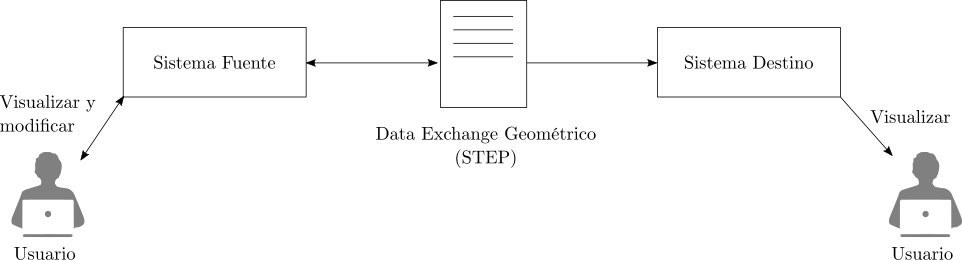
\includegraphics[width=14cm]{Img/WEB/de0.png}
\centering
\caption{\textbf{\footnotesize{Esquema de Data Exchange Geométrico con un archivo STEP a modo de ejemplo.}}}
\label{fig:de0}
\end{figure}

La mayoría de los sistemas CAD actuales soportan el paradigma de diseño basado en características, en inglés \textit{Feature Based} (FB), también llamado \textit{diseño paramétrico} y diseño basado en la historia como se explica en la sección \ref{cadparam}. Por lo tanto, es fundamental la incorporación del concepto de intercambio de datos basado en características, en inglés \textit{Feature Based Data Exchange} (FBDE) con el fin de dar soporte a los procesos de diseño colaborativos.\vskip
\textit{En el FBDE, dado un gráfico, basado en el historial paramétrico de un modelo (características) en un sistema origen, el objetivo es construir un gráfico en un sistema destino con una geometría similar, conservando al mismo tiempo la mayor información paramétrica posible}  \citep{SpitzRappoportA.b2004}. El FBDE conserva la inteligencia del diseño, permite que se realicen modificaciones en el lado del sistema destino como se puede observar en la Figura \ref{fig:de1} y ayuda a evitar el problema de las inconsistencias geométricas.\vskip

\begin{figure}[h]
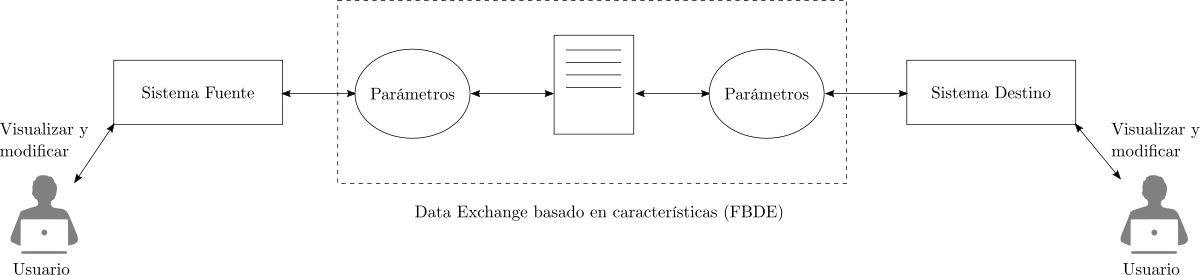
\includegraphics[width=16cm]{Img/WEB/de1.png}
\centering
\caption{\textbf{\footnotesize{Esquema de Data Exchange basado en características (FBDE).}}}
\label{fig:de1}
\end{figure}

En el paradigma de diseño basado en características, el modelo se representa como un árbol o lista de operaciones llamadas entidades, este árbol también se suele denominar ``árbol de historia". Las operaciones crean una nueva geometría o modifican la geometría existente. El punto principal de este paradigma es que las operaciones son de naturaleza paramétrica. En las Figuras \ref{fig:de2} y \ref{fig:de3} se puede ver un ejemplo práctico que ilustra el arbol de historia con las diferentes versiones de los modelos, desde el modelo original hasta el modelo objetivo. \vskip

\begin{figure}[h]
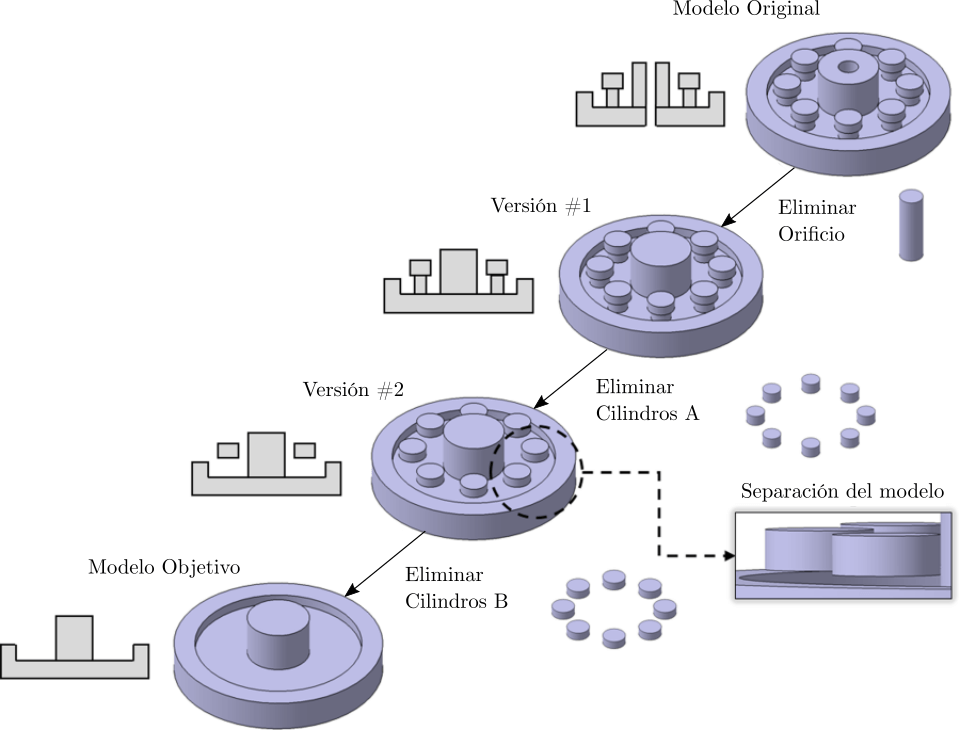
\includegraphics[width=14cm]{Img/WEB/de2.png}
\centering
\caption{\textbf{\footnotesize{Ejemplo de modificación de geometría}}}
\label{fig:de2}
\end{figure}

\begin{figure}[h]
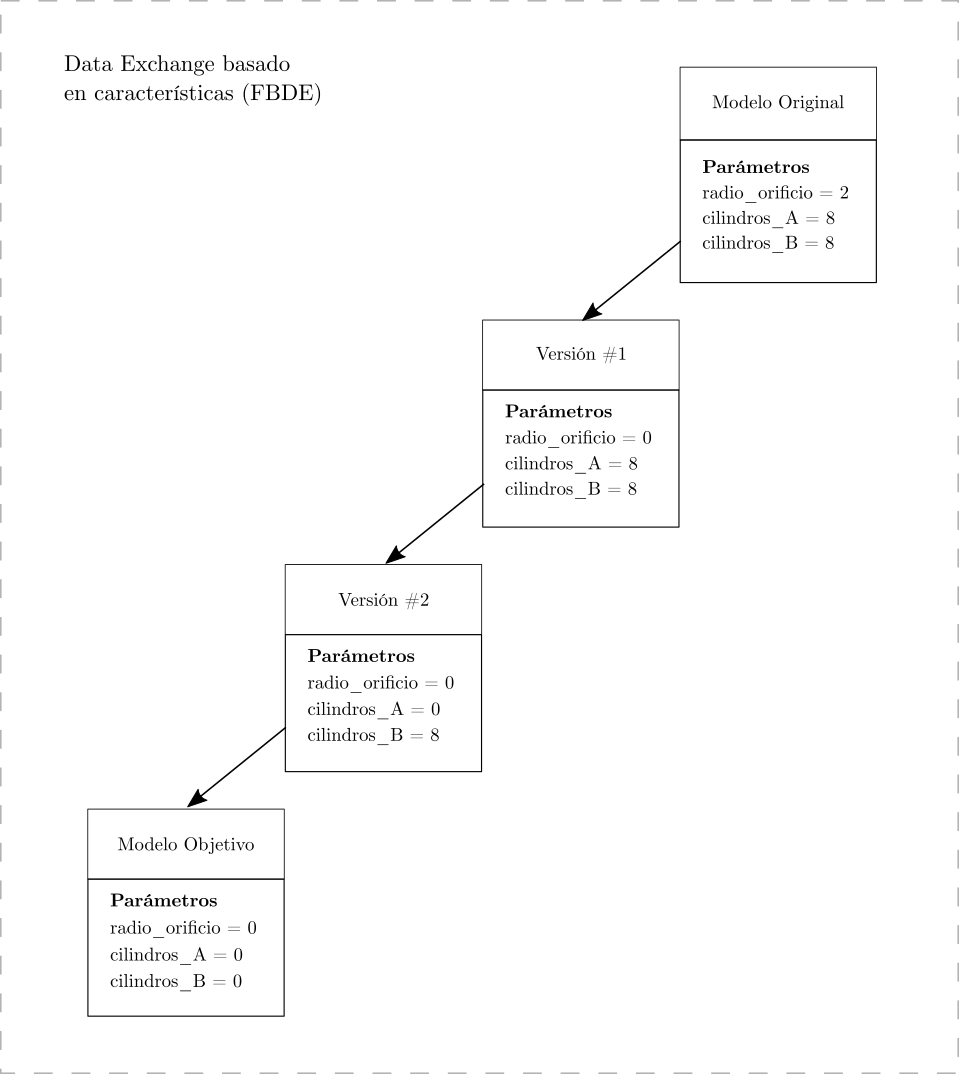
\includegraphics[width=14cm]{Img/WEB/de3.png}
\centering
\caption{\textbf{\footnotesize{Ejemplo de arbol de historia con las versiones de modelos y sus respectivos valores de los parámetros}}}
\label{fig:de3}
\end{figure}

El objetivo de FBDE es crear un modelo objetivo, empleando características en lo posible lo más similares al modelo original, es decir manteniendo la geometría. Es importante aclarar esto, porque en muchos casos, la geometría no puede ser idéntica debido a diferentes políticas de tolerancia entre los sistemas. Siempre que la aproximación esté controlada, este hecho es totalmente aceptable en la práctica.

\clearpage
\subsubsection{PDM Schema}
La Gestión de Datos del Producto , en inglés \textit{Product Data Management} (PDM) es una herramienta de productividad capaz de ayudar a un grupo de trabajo, departamento, división, o empresa en la gestión de datos del producto y del proceso de desarrollo a lo largo del ciclo de vida del producto, con el objetivo de mejorar considerablemente el flujo, calidad y uso de la información, facilitando así el control de datos, actividades, cambios y configuración del producto de ingeniería. \citep{Ruiz}\vskip
Por definición, un sistema PDM es ``algo" que maneja datos sobre productos. En el núcleo central de la información del PDM está la identificación del producto. Un producto es representado conceptualmente como un elemento o ítem dentro de la generalidad de un sistema PDM. \citep{Ungerer2002} \vskip

Un Esquema de PDM, en inglés \textit{PDM Schema} es una estructura o modelo de información de referencia para el intercambio o \textit{Data Exchange} de un subconjunto común de datos que se gestionan dentro de un sistema PDM. En el PDM Schema, el concepto general del producto se puede interpretar como uno o varios documentos. De esta forma, los documentos se pueden gestionar de forma coherente.\vskip

Los requisitos de gestión de datos del producto abordados por el PDM Schema se organizan en agrupaciones de conceptos relacionados. Estos grupos proporcionan una agrupación lógica de entidades o elementos con el propósito de una estructura clara.\vskip
La forma de agrupar elementos no es la misma en todos los sistemas. La agrupación depende de la dirección que tome el sistema general PDM, sus protocolos de aplicación, su alcance, etc. Por ejemplo: Para el PDM Schema establecido para promover la interoperabilidad entre sistemas que utilizan STEP, se recomienda una estructura modular, en sintonía con la dirección actual hacia la modularización de los contenidos técnicos de los recursos integrados STEP y sus protocolos de aplicación.

Las unidades modulares de funcionalidad para el PDM Schema del ejemplo se enumeran a continuación:

\begin{itemize}
    \item Identificación de la pieza
    \item Clasificación de la pieza
    \item Propiedades de la pieza
    \item Estructura de la pieza y relaciones
    \item Identificación del documento
    \item Clasificación del documento
    \item Archivos externos
    \item Relaciones entre documentos y archivos constitutivos
    \item Propiedades del documento y archivos
    \item Asociación de documentos y archivos a los datos del producto
    \item Relaciones entre documentos y archivos
    \item Identificación de alias
    \item Autorización
    \item Información de configuración y efectividad
    \item Datos de gestión del trabajo
\end{itemize}

A continuación se especifica un fragmento de un archivo de intercambio de datos en formato STEP para una pieza mecánica, con su contexto y tipo de clasificación. En el código se puede apreciar la estructura y modularización del PDM Schema.
\begin{minted}[baselinestretch=1, bgcolor=LightGray]{HTML}

ISO-10303-21; 
HEADER; 
FILE_DESCRIPTION(('test', 'file'), '2;1');
FILE_NAME('pid2_p21a.stp', '1999-05-03T21:03:29+00:00', ('N.N.'),
(''), '', '', ''); 
FILE_SCHEMA(('PDM_SCHEMA {1.2})); 
ENDSEC; 
DATA;
/* Pieza #1 */ 
#10 = PRODUCT('K01-42051', 'Bicicleta Bell RX 3', $, (#20));

/* Contexto de la Pieza */ 
#20 = PRODUCT_CONTEXT('', #30, ''); 
#30 = APPLICATION_CONTEXT(''); 
#40 = APPLICATION_PROTOCOL_DEFINITION('version 1.2', 'pdm_schema',
2000, #30);

/* Versiones para la Pieza #1 */ 
#50 = PRODUCT_DEFINITION_FORMATION('02', 'Palanca modificada',
#10); #60 = PRODUCT_DEFINITION_FORMATION('03', '
Carcasa superior modificada', #10); 
#70 = PRODUCT_DEFINITION_FORMATION_RELATIONSHIP('', 'sequence', $,
#50, #60);

/* Definicion de la vista versión 03 de la Pieza #1 */ 
/* primary life_cycle_stage = diseño, 
primary application_domain = diseño mecánico */ 

#80 = PRODUCT_DEFINITION('/NULL', $, #60, #90); #90 =
PRODUCT_DEFINITION_CONTEXT('part definition', #100, 'design');
#100 = APPLICATION_CONTEXT('diseño mecánico');

/* Asociación del usuario id a la Pieza #1 */ #130 =
APPLIED_ORGANIZATION_ASSIGNMENT(#140, #150, (#10, #160, #170));
#150 = ORGANIZATION_ROLE('id owner');

/* Informacion de la persona y la organizacion */ 
#140 = ORGANIZATION('ABC27166', 'Misiones Argentina', 'location');
#540 = PERSON('nombre@email.com', 'Pedro', 'Perez', $, $, $);
#550 = PERSON_AND_ORGANIZATION(#540, #140);

/* Pieza #2 y Pieza #3 */ 
#160 = PRODUCT('H24-1123.1', 'Fixture RX25B', '', (#20)); 
#170 = PRODUCT('DIN 932', 'Screw M3x15', '', (#20));

/* Versiones para Pieza #2 y Pieza #3 */ 
#180 = PRODUCT_DEFINITION_FORMATION('B', 'agujeros para tornillos
más grandes', #160); 
#190 = PRODUCT_DEFINITION_FORMATION('15', '', #170);

/* Definición de las vistas para versión de Pieza #2 */ 
#200 = PRODUCT_DEFINITION('/NULL', $, #180, #210); 
#210 = PRODUCT_DEFINITION_CONTEXT('part definition',
#215, 'diseño'); #215 = APPLICATION_CONTEXT('diseño mecánico');

/* Definición de las vistas para versión de Pieza #3 */ 
#220 = PRODUCT_DEFINITION('/NULL', $, #190, #230); 
#230 = PRODUCT_DEFINITION_CONTEXT('part definition', #240, 'diseño'); 
#240 = APPLICATION_CONTEXT('diseño mecánico');
...
ENDSEC; END-ISO-10303-21;
\end{minted}



\subsubsection{Data Exchange en entornos web}

En la actualidad los sistemas PDM están aprovechando las posibilidades que ofrece internet. Este nuevo enfoque permite el trabajo entre personas establecidas en distintos puntos geográficos, gracias a la posibilidad de acceso remoto a las bases de datos. 
Con estos nuevos sistemas es posible la utilización del PDM por parte de múltiples especialistas implicados en el desarrollo de un producto, permitiendo que esta tecnología sea una plataforma de integración entre los interesados y una excelente ayuda para la puesta en marcha y tareas de soporte.

XML fué por mucho tiempo el formato estándar de facto para el intercambio de datos en el contexto de las aplicaciones de servicios web, en inglés \textit{web services}. Sin embargo, en comparación con XML, JSON es un formato de intercambio de datos mucho más ligero. Esta distinción es importante, ya que la eficiencia en la asignación de datos entre diferentes modelos de datos es el punto clave para mejorar el rendimiento de las aplicaciones basadas en web services. \citep{Zunke2014}

A continuación se explica brevemente los dos formatos más utilizados para Data Exchange en contextos web, el tradicionalmente utilizado (XML) y (JSON) comparativamente nuevo, sus objetivos de diseño y sus características fundamentales.

\subsubsection{XML}

XML\footnote{\url{https://www.w3.org/XML/}} o Extensible Markup Language es un conjunto de estándares publicados por XML Working Group en el Consorcio World Wide Web  (W3C), el grupo que regula los estándares de Internet (www). Básicamente, un documento XML se compone de algunas etiquetas, en inglés \textit{tags} bien definidas y los datos incluidos en ellas. Las etiquetas son contenedores que describen los datos adjuntos y también los organizan. Los objetivos de diseño para XML v1.1 publicados en la recomendación W3C son los siguientes:

\begin{itemize}
    \item XML se podrá usar directamente en Internet.
    \item XML debe admitir una amplia variedad de aplicaciones.
    \item XML debe ser compatible con SGML.
    \item Será fácil escribir programas que procesen documentos XML.
    \item El número de características opcionales en XML debe mantenerse en el mínimo absoluto, idealmente cero.
    \item Los documentos XML deben ser legibles por los humanos y razonablemente claros.
    \item El diseño de XML debe prepararse rápidamente.
    \item El diseño de XML debe ser formal y conciso.
    \item Los documentos XML deben ser fáciles de crear.
    \item La rigidez en el marcado XML es de mínima importancia.
\end{itemize}

La especificación de sintaxis y las regulaciones con respecto a la correcta forma de un documento XML se pueden consultar en la especificación W3C para XML v1.1

\begin{minted}[baselinestretch=1, bgcolor=LightGray]{HTML}
<?xml version="1.1"?> 
    <greeting>Hola Mundo!</greeting> 
<!--Esto es un comentario -->
\end{minted}
\begin{center}
    \caption{Ejemplo de un documento XML}    
\end{center}



\subsubsection{JSON}
JSON o Javascript Object Notation es un formato de datos basado en texto ligero y diseñado para que los datos sean legibles por humanos, el formato ha sido popularizado por Douglas Crockford.  Aunque es muy parecido a la sintaxis de objeto literal de JavaScript, puede ser utilizado independientemente de JavaScript.

JSON está constituído por dos estructuras:

\begin{itemize}
    \item Una colección de pares de nombre/valor. En varios lenguajes esto es conocido como un objeto, registro, estructura, diccionario, tabla hash, lista de claves o un arreglo asociativo.
    \item Una lista ordenada de valores. En la mayoría de los lenguajes, esto se implementa como arreglos, vectores, listas o sequencias.
\end{itemize}

Estas son estructuras universales; virtualmente todos los lenguajes de programación las soportan de una forma u otra. Por ende, es razonable que un formato de intercambio de datos que es independiente de los lenguajes de programación se base en estas estructuras.

\begin{minted}[baselinestretch=1, bgcolor=LightGray]{HTML}
{ "greeting": "Hola Mundo!" } 
\end{minted}
\begin{center}
\caption{Ejemplo de objeto JSON}
\end{center}

\subsubsection{Comparación de características}
En esta sección se analizan las características más destacadas de ambos formatos.

\begin{enumerate}
    \item \textbf{Adopción en la Industria}
    \begin{itemize}
        \item XML ha sido el estándar de la industria por mas de una década y tiene muchos apoyo gracias a los estándares.
        \item JSON, por otro lado, si bien es ampliamente utilizado, no tiene estándares como Schematrons, XSD.
    \end{itemize}
    
    \item \textbf{Metadatos}
    \begin{itemize}
        \item XML tiene una gran sobrecarga en forma de metadatos por el uso de etiquetas \textless \textgreater.
        \item JSON tiene metadatos mínimos que lo hacen muy compacto.
    \end{itemize}
    
    \item \textbf{Soporte de framework}
    \begin{itemize}
        \item XML es compatible con la mayoría de las implementaciones de framework (API) en toda la industria.
        \item Al principio JSON no tenía mucho soporte, sin embargo pero se ha posicionado muy rápido en términos de adopción.
    \end{itemize}
    
    \item \textbf{Extensibilidad}
    \begin{itemize}
        \item XML permite almacenar cualquier tipo de datos. Los atributos del elemento de datos permiten flexibilidad adicional.
        \item JSON está limitado solo al almacenamiento de datos clásicos como texto y números.
    \end{itemize}
    
    \item \textbf{Facilidad de mapeo}
    \begin{itemize}
        \item XML está orientado a documentos (estructura de árbol), lo que dificulta su asignación a objetos en el paradigma de programación orientado a objetos (OOP).
        \item JSON está orientado a datos, por lo tanto, está más cerca de la estructura de los objetos en el paradigma de OOP.
    \end{itemize}
    
    \item \textbf{Rendimiento}
    \begin{itemize}
        \item Debido a la sobrecarga de metadatos, los datos requiere, de más ancho de banda si se expresan en XML.
        \item Los datos en JSON son muy compactos, utilizando la menor cantidad de ancho de banda.
    \end{itemize}
    
\end{enumerate}


\subsubsection{Análisis de rendimiento (Benchmark)}
Para el análisis y la comparación del rendimiento, ambos formatos de datos (XML y JSON) se comparan respecto al uso de memoria y los tiempos de ejecución en los siguientes experimentos realizados por el \textit{Vishwakarma Institute of Information Technology} de la universidad de Pune en la India.
\begin{enumerate}
    \item Serialización o marshaling desde un objeto Java a una secuencia de memoria almacenada (buffer) sin compresión.
    \item Serialización o marshaling desde un objeto Java a una secuencia de memoria almacenada (buffer) con compresión.
    \item Des-serialización o unmarshaling de una secuencia de memoria almacenada (buffer) a un objeto Java.
\end{enumerate}

Las pruebas de rendimiento se realizaron ejecutando 100 muestras para cada experimento y 100 instancias de cada experimento. A continuacion se pueden ver muestras generadas de archivos XML y JSON respectivamente.

\begin{minted}[baselinestretch=1, bgcolor=LightGray]{HTML}
<?xml version="1.0" encoding="UTF-8" ?> 
<Hotel xmlns="http://www.example.org/Hotel">
    <hotelID>15013</hotelID>
    <hotelName>rhhjwhuqabhpitcewkrc</hotelName> 
    <menu> 
        <food> 
            <name>wdppncqtkhubtvkagpvm</name> 
            <price>48161</price> 
            <calories>49311</calories>
        </food>
    </menu>
</Hotel>
\end{minted}
\begin{center}
\caption{Archivo XML de muestra generado aleatoriamente}
\end{center}

\begin{minted}[baselinestretch=1, bgcolor=LightGray]{HTML}
{"hotelID":80814, "hotelName":"glovcnbwaviboawddgvx", 
"menu":
{"food":[{"name":"fprgunyzwvjkruwalbny",
"price":63463,"calories":95471}]}}
\end{minted}
\begin{center}
\caption{Archivo JSON de muestra generado aleatoriamente}
\end{center}



En lo que respecta al rendimiento, el formato de intercambio de datos JSON es el claro ganador entre los dos. Tanto en términos de uso de memoria como de tiempo de ejecución, JSON ofrece un mejor rendimiento. Incluso con la compresión habilitada, XML produjo mucho más sobrecarga en la secuencia de datos que JSON.

La siguiente tabla resume las medidas concluyentes de los experimentos:

\begin{center}
 \begin{tabular}{ | c | c | c | c |} 
   \hline
   Aspectos de rendimiento & JSON & XML & JSON/XML  \\ 
   \hline
   Tamaño de Secuencia (sin comprimir) & 137B & 279B & 49\% \\
   \hline
   Tamaño de Secuencia (comprimido) & 133B & 219B & 61\% \\
   \hline
   Consumo en la Serialización & 3312B & 22128B & 15\% \\
   \hline
   Consumo en la Des-serialización & 5840B & 7040B & 83\% \\
   \hline
   Tiempo de Serialización (sin comprimir) & 11614ns & 23591ns & 49\% \\
   \hline
   Tiempo de Serialización (comprimido) & 9884ns & 19310ns & 51\% \\
   \hline
   Tiempo de Des-serialización & 13880ns & 43595ns & 32\% \\
   \hline
 
\end{tabular}
\end{center}
\begin{center}
\caption{Medidas concluyentes de los experimentos}
\end{center}

XML se puede usar como data exchange si:
\begin{itemize}
    \item El rendimiento de la aplicación no es la principal prioridad.
    \item Se puede permitir que el consumo de memoria de una aplicación sea grande.
    \item Es necesario que haya un estricto cumplimiento de un protocolo estándar para la comunicación.
    \item La optimización de los datos enviados a través de la red no es prioridad.
\end{itemize}

Por el contrario, JSON se puede utilizar como data exchange si:
\begin{itemize}
    \item El rendimiento de la aplicación es una consideración de diseño.
    \item El tiempo de utilización de memoria de una aplicación debe mantenerse muy pequeño o mínimo.
    \item Puede haber una desviación sobre el formato de comunicación entre las partes o bien las partes pueden ponerse de acuerdo para realizar los cambios en el formato cuando sea necesario.
    \item Los datos enviados a través de la red deben optimizarse.
\end{itemize}

\subsubsection{JSON como FBDE}
Anteriormente se realiza un análisis de JSON comparado con XML, es importante destacar que la popularidad de JSON se debe en gran parte a la compatibilidad nativa que tiene este formato con muchos sistemas de gestión de bases de datos (DBMS). Las bases de datos relacionales como PostgreSQL\footnote{\url{https://www.postgresql.org/}} y MySQL\footnote{\url{https://www.mysql.com/}} actualmente incluyen soporte nativo para almacenar y consultar datos JSON. Las bases de datos NoSQL\footnote{\url{https://aws.amazon.com/es/nosql/}} como MongoDB\footnote{\url{https://www.mongodb.com/}} también son compatibles con JSON, aunque MongoDB utiliza una versión ligeramente modificada de JSON. MongoDB representa documentos JSON en un formato codificado en binario llamado BSON\footnote{\url{https://www.mongodb.com/json-and-bson}}. BSON amplía el modelo de JSON para proporcionar algunos tipos de datos adicionales, el uso de campos ordenados y eficiencia para la codificación y decodificación en diferentes lenguajes.\vskip
Si se desarrolla un software que se comunica con un navegador web o una aplicación móvil, la recomendación es usar JSON como formato de datos de intercambio. Usar un formato como XML se considera una opción desactualizada.\vskip
JSON en la actualidad es el formato mas recomendado para enviar datos entre servidores web y navegadores. Su diseño simple y su flexibilidad hacen que sea fácil de leer y comprender, y en la mayoría de los casos, fácil de manipular para los lenguajes de programación. La falta de un esquema estricto permite la flexibilidad del formato, aunque esa flexibilidad a veces hace que sea difícil garantizar que esté leyendo y escribiendo JSON correctamente. \citep{EddieSmith2018} \vskip

Para dar soporte a los procesos colaborativos, es necesario que los archivos JSON puedan incluir especificaciones de diseños basadas en características. Es decir, los archivos JSON deben soportar el intercambio de datos basados en características (FBDE) y contar con estructuras para especificar el ``arbol de historia" de un modelo. En el contexto de este trabajo y para el desarrollo del prototipo COCADA, se recomienda el uso de JSON como FBDE.\vskip
Respecto a la estructura del PDM Schema a utilizar en este trabajo, es importante aclarar que se limita al ámbito de aplicación y no incorporan todos los contenidos que se utilizan en otros PDM Schema de uso general como puede ser STEP.\vskip
El PDM Schema tentativo para COCADA incluye entre otras, las siguientes unidades modulares:
\begin{itemize}
    \item Identificación del diseño o proyecto
    \item Árbol de historia
    \item Geometría de un objeto en la historia
    \item Usuarios
    \item Relación de un usuario a la historia
    \item Parámetros de un objeto en la historia
    \item Archivos adjuntos
    \item Relación de archivos adjuntos con proyecto.
    \item Conversaciones de usuarios
    \item Relación de conversaciones con la historia
\end{itemize}


\clearpage
\section{Trabajos relacionados}
A continuación se detallan algunas herramientas existentes que poseen características similares al prototipo COCADA. 
En la explicación de estas tecnologías se pueden apreciar algunas diferencias respecto al prototipo planteado en este trabajo, tanto en la representación de los modelos como en la gestión de la información. De todas maneras, estas herramientas son antecedentes de gran valor porque aportan ideas de gran utilidad para posibles soluciones, sobre todo en las áreas de experiencia de usuario UX y diseño UI\footnote{UI o interfaz de usuario es el espacio donde se producen las interacciones entre seres humanos y máquinas.}.

\subsection{Customizer}
Customizer\citep{MakerBot2018} es una aplicación web desarrollada por la empresa Makerbot\footnote{\url{https://www.makerbot.com/}} y disponible en Thingiverse\footnote{\url{https://www.thingiverse.com/}}, una plataforma para publicación de diseños  especializada en impresión 3D.

Customizer permite adjuntar o subir a la aplicación archivos de código OpenSCAD. En éstos se especifican modelos 3D paramétricos con la definición de sus variables.

Luego procesa el código OpenSCAD, analiza las variables y agrega los elementos o controles UI correspondientes, como barras deslizantes, botones de opciones, etc.\vskip 

Mediante la modificación de los parámetros por medio de los controles UI se pueden generar objetos sólidos personalizados. En la Figura \ref{fig:customizer} se puede ver la interfaz.

Customizer es una manera sencilla de generar diseños colaborativos mediante la personalización de modelos 3D por parte de la comunidad de usuarios de la plataforma Thingverse.

\begin{figure}[h]
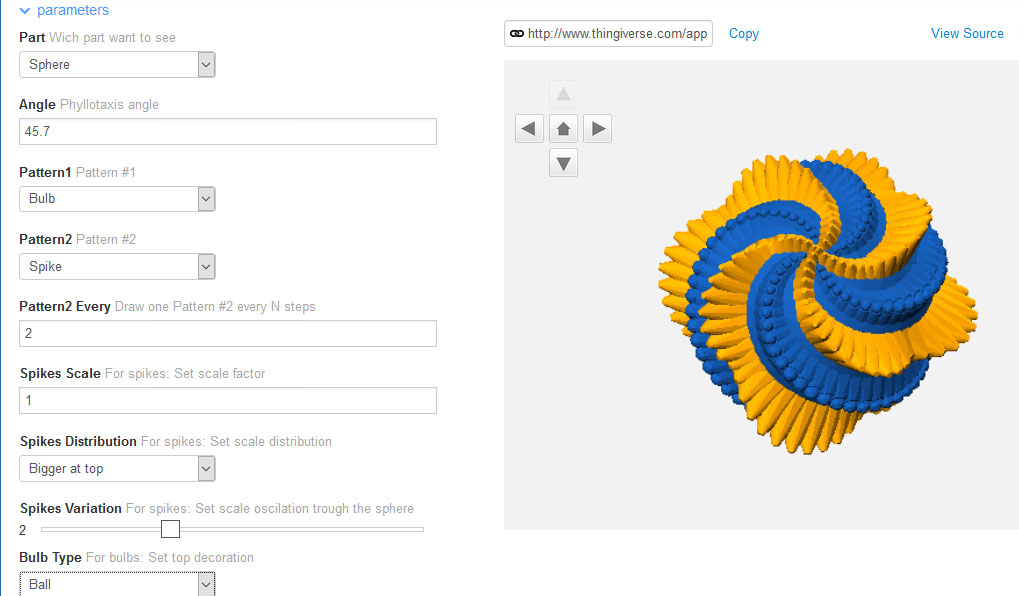
\includegraphics[width=14cm]{Img/WEB/web-maker.jpg}
\centering
\caption{\textbf{ \footnotesize{Interfaz de Customizer con un objeto y sus parametros}}}
\label{fig:customizer}
\end{figure}

\subsection{Beta.Spekle}

Spekle\citep{UCL2018} es un proyecto desarrollado por \textit{The Bartlett School of Architecture UCL}\footnote{\url{https://www.ucl.ac.uk/bartlett/architecture/}} pensado para que los usuarios de Grasshopper puedan compartir diseños paramétricos en la web. 
El proyecto consta de:
\begin{itemize}
    \item Un plugin Spekle, que en combinación con Grasshopper permite establecer los parametros de los modelos y exportarlos a archivos SPK para luego visualizarlos en la web. En la Figura \ref{fig:plugin} se puede ver un ejemplo de uso.
    \item Una aplicación web que permite subir archivos SPK para visualizar los modelos paramétricos con sus respectivas variables, crear versiones modificadas y registrar un historial de los cambios en los modelos. Ver \ref{fig:spekle}
\end{itemize}

\textbf{Beta.Spekle}\footnote{\url{http://beta.speckle.xyz/}} es la versión de desarrollo de la plataforma web y se publica como un proyecto FLOSS que acepta contribuciones de la comunidad.

\begin{figure}[h]
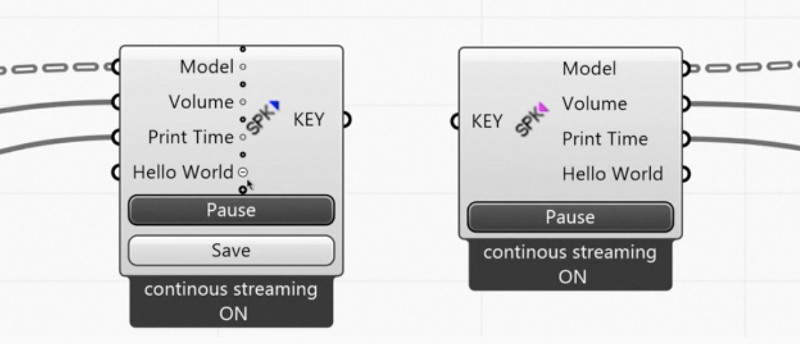
\includegraphics[width=8cm]{Img/WEB/web-plugin.jpg}
\centering
\caption{\textbf{ \footnotesize{Uso de Spekle junto a Grasshopper.}}}
\label{fig:plugin}
\end{figure}

\begin{figure}[h]
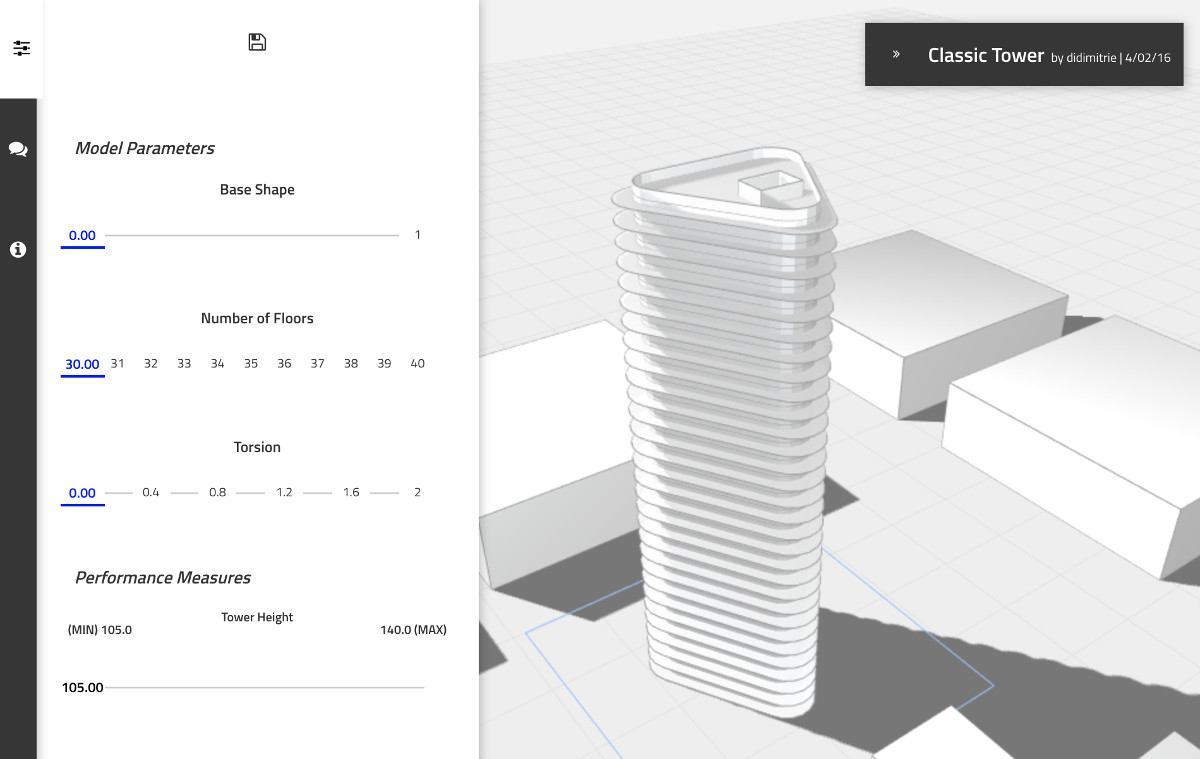
\includegraphics[width=14cm]{Img/WEB/web-spekle.jpg}
\centering
\caption{\textbf{ \footnotesize{Interfaz de beta.spekle, a la izquierda se pueden apreciar los parámetros del modelo.}}}
\label{fig:spekle}
\end{figure}


\subsection{Modelo.io}

Modelo.io\citep{Modelo.io2018} es una plataforma web creada por Qi Su y Tian Deng, orientada a profesionales que trabajan con software CAD como Rhino\footnote{\url{https://www.rhino3d.com/es}} y SketchUp\footnote{\url{https://www.sketchup.com/es}}. Permite una colaboración intuitiva entre los miembros de un equipo para perfeccionar los diseños y presentarlos de forma interactiva.

Mediante modelo, los usuarios visualizan y exploran diseños en 3D, proporcionan comentarios, almacenan archivos de proyectos, se comunican entre los miembros del equipo y puedan crear presentaciones 3D interactivas para los clientes. En la Figura \ref{fig:modelo.io} se puede ver la interacción de usuarios.

La características más llamativas que incluyen son los recorridos virtuales para arquitectura y la visualización de escenas en realidad virtual.

El servicio ofrece una versión reducida, gratuita para estudiantes registrados. Para acceder a todas las funcionalidades de modelo.io las cuentas son de servicio pago.

\begin{figure}[h]
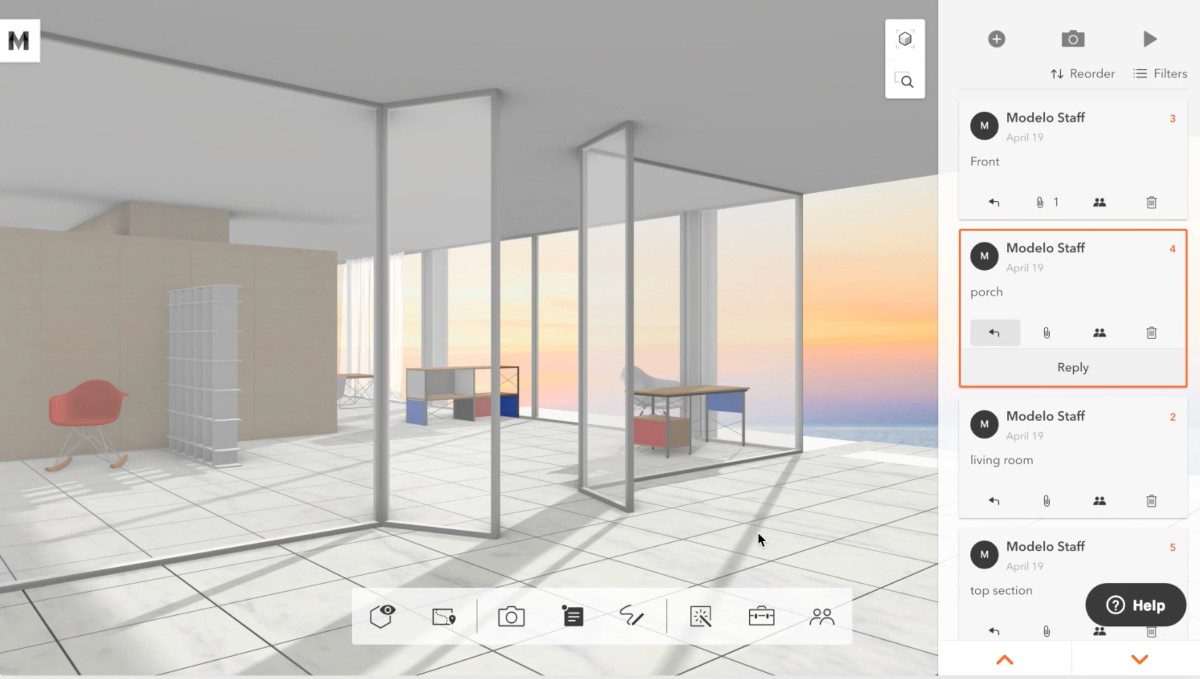
\includegraphics[width=14cm]{Img/WEB/web-modelo.jpg}
\centering
\caption{\textbf{ \footnotesize{Interfaz de Modelo.io, a la derecha se puede apreciar la interacción entre usuarios.}}}
\label{fig:modelo.io}
\end{figure}